%%%%%%%%%%%%%%%%%%%%%%%%%%%%%%%%%%%%%%%%%%%%%%%%%%%%%%%%%%
% ĐÂY LÀ FILE CHÍNH (main.tex)
% File này quản lý toàn bộ cài đặt và gọi các chương con
%%%%%%%%%%%%%%%%%%%%%%%%%%%%%%%%%%%%%%%%%%%%%%%%%%%%%%%%%%

\documentclass[notheorems,hyperref={bookmarks=true}]{beamer}
\usepackage[framesassubsections]{beamerprosper}
\hypersetup{pdfpagemode=FullScreen}
\usepackage[utf8]{vietnam}
%\usepackage[tcvn]{vietnam}
\usepackage[english]{babel}
\usepackage{ulem} %for underlying+
\usepackage{pifont} %for creating dingautolist
\usepackage[mathscr]{eucal}
\usepackage{amsmath, amsthm, amssymb,amsxtra,latexsym,amscd,graphics,graphpap}
\usepackage{indentfirst}
\usepackage{rotating}
\usepackage{graphicx}
\usepackage{amsbsy}
\usepackage{epsfig}
\usepackage{natbib}
%\usepackage{pst-plot}
%\usepackage{msc}
%\usepackage{musixtex}
% --- ĐẢM BẢO CÁC GÓI NÀY CÓ TRONG main.tex ---
\usepackage{mathtools}  % Cần cho 'phan3_chuong1.tex' [cite: 52]
\usepackage{amsfonts}   % Cần cho \mathbb{} [cite: 52]
\usepackage{amsbsy}     % Cần cho \boldsymbol

\usepackage{pdfpages}
\usepackage{multicol}
\usepackage{hyperref}
\usepackage{subfigure}
\usepackage{multimedia}
\usepackage{boxedminipage}
\usepackage{tikz}
\usepackage{nicefrac}
\usepackage{diagbox}
\usepackage{graphicx}
\setbeamertemplate{theorems}[numbered] % Đánh số định lý.

% --- THÊM CÁC GÓI NÀY VÀO main.tex ---
\usepackage{mathtools}  % Gói mới (bổ sung cho amsmath)
\usepackage{arydshln}   % Gói mới (để vẽ đường nét đứt trong bảng)
\usepackage{bm}
\usepackage{amsfonts}   % Gói mới (cho \mathbb)

% --- THÊM CÁC LỆNH NÀY VÀO main.tex (khu vực \providecommand) ---
\newcommand{\E}{\mathbb{E}}
\newcommand{\Var}{\mathrm{Var}}
\newcommand{\Cov}{\mathrm{Cov}}

% --- CÀI ĐẶT THEME VÀ MÀU SẮC ---
% (Giữ nguyên toàn bộ cài đặt của bạn)
\usetheme{Copenhagen}
\usecolortheme{rose} 
\setbeamertemplate{headline}{}
\usefonttheme[onlylarge]{structurebold}
\usefonttheme{professionalfonts}

\setbeamercolor{title}{fg=red!80!black,bg=blue!20!white}
\setbeamertemplate{section in head/foot shaded}[default][20]
\setbeamertemplate{subsection in head/foot shaded}[default][20]
\setbeamertemplate{navigation symbols}{}
\setbeamertemplate{blocks}[rounded][shadow=true]
\setbeamerfont{small}{size=\small}
\setbeamerfont{footnote}{size=\footnotesize}
\setbeamerfont{script}{size=\scriptsize}
\setbeamerfont{tiny}{size=\tiny}

% --- CÁC LỆNH TẮT VÀ MÔI TRƯỜNG ---
\providecommand{\R}{\mathbb{R}}
\providecommand{\Mat}{\textsc{MatLab }}
\providecommand{\lr}[1]{\left( #1 \right)} 
\providecommand{\Lr}[1]{\left[ #1 \right]}
\providecommand{\LR}[1]{\left\{ #1 \right\}} 
\providecommand{\abs}[1]{\left\vert #1 \right\vert} 
\providecommand{\norm}[1]{\left\Vert #1 \right\Vert} 
\providecommand{\ov}[1]{\overline {#1}} 
\providecommand{\e}{\varepsilon} 
\DeclareMathSymbol{\INT}{\mathop}{largesymbols}{"5A} 
\renewcommand{\int}{\INT} 
\renewcommand{\iint}{\mathop{\int\!\!\!\!\!\int}}
\renewcommand{\iiint}{\mathop{\int\!\!\!\!\!\int\!\!\!\!\!\int}}
\DeclareMathOperator{\sinc}{sinc}

\theoremstyle{plain}
%\theorembodyfont{\slshape}
\newtheorem{definition}{Định nghĩa}[section]
\newtheorem{proposition}{Mệnh đề}[section]
\newtheorem{theorem}{Định lý}[section]
\newtheorem{lemma}{Bổ đề}[section]
\newtheorem{corollary}{Hệ quả}[section]
\newtheorem{conjecture}{Dự đoán}[section]
\newtheorem{remark}{Chú ý}[section]
\newtheorem{example}{Ví dụ}
\newtheorem{problem}{Bài toán}[section]
\newtheorem{exercise}{Bài tập}

\renewcommand{\thedefinition}{\arabic{section}.\arabic{definition}}
\renewcommand{\thelemma}{\arabic{section}.\arabic{lemma}}
\renewcommand{\thetable}{\Roman{table}}
\renewcommand{\thetheorem}{\arabic{section}.\arabic{theorem}}
\renewcommand{\thecorollary}{\arabic{section}.\arabic{corollary}}
\renewcommand{\theequation}{\arabic{section}.\arabic{equation}} 
\renewcommand{\thefootnote}{(\arabic{footnote})}
\renewcommand{\theexample}{\arabic{example}}
\renewcommand{\theproblem}{\arabic{section}.\arabic{problem}}
\renewcommand{\theexercise}{\arabic{exercise}}
\mode<presentation>
\setbeamertemplate{navigation symbols}{} 

% --- LOGO ---
\pgfdeclareimage[height=1cm]{fami-logo}{Logo-khoa-chup}
%\pgfdeclareimage[height=1.5cm]{hust-logo}{logo}
\logo{\pgfuseimage{fami-logo}}

% --- THÔNG TIN TRANG BÌA CHÍNH ---
% (Bạn hãy thay đổi các thông tin này cho phù hợp với đề tài)
\title[Phân tích số liệu]{TÊN ĐỀ TÀI BÁO CÁO CỦA NHÓM BẠN} 
\author[Nhóm X]{Thành viên 1 \and Thành viên 2 \and Thành viên 3} 
\institution[SAMI-HUST]{Khoa, ĐHBK Hà Nội}
\date{Hà Nội, tháng 11 năm 2025}

\renewcommand{\sfdefault}{cmss}
\renewcommand{\rmdefault}{cmr}
\renewcommand{\ttdefault}{cmtt}

%%%%%%%%%%%%%%%%%%%%%%%%%%%%%%%%%%%%%%%%%%%%%%%%%%%%%%%%%%
% BẮT ĐẦU NỘI DUNG BÀI BÁO CÁO
%%%%%%%%%%%%%%%%%%%%%%%%%%%%%%%%%%%%%%%%%%%%%%%%%%%%%%%%%%
\begin{document}
\begin{footnotesize} % Mở môi trường chữ nhỏ (lấy từ code của bạn)

% --- SLIDE TIÊU ĐỀ (TRANG BÌA) ---
\begin{frame}
	\frametitle{}
	\maketitle
\end{frame}

% --- SLIDE MỤC LỤC TỔNG ---
% (Slide này sẽ tự động hiện 5 chương của bạn)
\begin{frame}
	\frametitle{Nội dung chính}
	\tableofcontents
\end{frame}

% --- TỰ ĐỘNG TẠO MỤC LỤC CHO TỪNG PHẦN ---
% (Giữ nguyên code này của bạn)
%\AtBeginSection[] 
%{
	%\begin{frame}<beamer>
		%\frametitle{Nội dung}
		%\tableofcontents[currentsection, currentsubsection]
	%\end{frame}
%}


%%Chương 1 ĐANG LỖI
\section{Ước lượng Khoảng của Mô hình Hồi quy Tuyến tính}

%-------------------------------------------------------------------------------
% SLIDE 1: Giới thiệu Chương 4 & Bài toán (Trước 4.1)
%-------------------------------------------------------------------------------
\begin{frame}{Chương 4: Ước lượng Khoảng - Đặt vấn đề}

    \begin{itemize}
        \item \textbf{Bài toán:} Sau khi ước lượng điểm các hệ số hồi quy $\hat{\beta}$ và phương sai sai số $s^2$, ta cần:
        \begin{enumerate}
            \item Xác định độ tin cậy của các ước lượng này ($\beta$ và $\sigma^2$).
            \item Kiểm tra các giả thuyết về mối quan hệ tuyến tính giữa các biến.
        \end{enumerate}
        
        \item \textbf{Cơ sở lý thuyết:} Để thực hiện suy luận, ta cần bổ sung giả định:
        \[
            Y = Z\beta + \epsilon, \quad \text{với } \epsilon \sim \mathcal{N}_n(0, \sigma^2 I)
        \]
    \end{itemize}
\end{frame}

%-------------------------------------------------------------------------------
% SLIDE 2: Định lý 4.1 - Phân phối
%-------------------------------------------------------------------------------
\begin{frame}{Định lý 4.1: Phân phối của Ước lượng $\hat{\beta}$ và $RSS$}

    \begin{block}{Phát biểu Định lý 4.1}
        Xét mô hình hồi quy tuyến tính cổ điển $Y=Z\beta+\epsilon$ với ma trận $Z$ đầy hạng và $\epsilon \sim \mathcal{N}_n(0,\sigma^2I)$.
        Khi đó:
        \begin{itemize}
            \item $\hat{\beta}=(Z^{\prime}Z)^{-1}Z^{\prime}Y\sim\mathcal{N}_{r+1}(\beta,\sigma^{2}(Z^{\prime}Z)^{-1})$
            \item $n\hat{\sigma}^{2}=\hat{\epsilon}^{\prime}\hat{\epsilon}\sim\sigma^{2}\chi_{n-r-1}^{2}$
            \item $\hat{\beta}$ và $\hat{\epsilon}$ là hai biến độc lập
        \end{itemize}
    \end{block}
\end{frame}

%-------------------------------------------------------------------------------
% SLIDE 3: Chứng minh 4.1 (Ý tưởng) & Quy ước s^2
%-------------------------------------------------------------------------------
\begin{frame}{Chứng minh Định lý 4.1 (Phần 1/3)}
    \framesubtitle{Phân phối của Ước lượng Hệ số Hồi quy $\hat{\beta}$}

     \begin{itemize}
        \item \textbf{Cơ sở}: $\hat{\beta}$ là tổ hợp tuyến tính của vector biến chuẩn $\epsilon \sim \mathcal{N}_n(0, \sigma^2 I)$, nên $\hat{\beta}$ cũng là chuẩn.
        \item \textbf{Biểu diễn $\hat{\beta}$}: Ta có $\hat{\beta} = (Z'Z)^{-1}Z'Y$. Thay $Y = Z\beta + \epsilon$ vào:
        \[
            \hat{\beta} = (Z'Z)^{-1}Z'(Z\beta + \epsilon) = \beta + (Z'Z)^{-1}Z'\epsilon
        \]

        \item \textbf{Kỳ vọng $E(\hat{\beta})$} (Giá trị trung bình):
        \[
            E(\hat{\beta}) = E\left(\beta + (Z'Z)^{-1}Z'\epsilon\right) = \beta + (Z'Z)^{-1}Z'E(\epsilon) = \beta
        \]
        (Vì $E(\epsilon) = 0$).
        \item \textbf{Phương sai $Cov(\hat{\beta})$} (Tính bất định):
        \begin{align*}
            Cov(\hat{\beta}) &= Cov\left((Z'Z)^{-1}Z'\epsilon\right) \\
            &= (Z'Z)^{-1}Z' \cdot Cov(\epsilon) \cdot Z(Z'Z)^{-1} \\
            &= (Z'Z)^{-1}Z' (\sigma^2 I) Z(Z'Z)^{-1} \\
            &= \sigma^2 (Z'Z)^{-1} (Z'Z) (Z'Z)^{-1} = \sigma^2 (Z'Z)^{-1}
        \end{align*}
        
        \textbf{Kết luận}: $\hat{\beta} \sim \mathcal{N}_{r+1}(\beta, \sigma^2 (Z'Z)^{-1})$.
    \end{itemize}
\end{frame}

\begin{frame}{Chứng minh Định lý 4.1 (Phần 2/3)}
    \framesubtitle{Phân phối $\chi^2$ của $\hat{\epsilon}'\hat{\epsilon}$ (Tổng Bình phương Sai số)}

    \begin{itemize}
        \item \textbf{Biểu diễn $\hat{\epsilon}$}: Sai số ước lượng là $\hat{\epsilon} = Y - \hat{Y} = (I - H)Y$.
        Thay $Y = Z\beta + \epsilon$:
        \[
            \hat{\epsilon} = (I - H)(Z\beta + \epsilon) = (I - H)\epsilon
        \]
        (Vì $Z\beta = HZ\beta = H\hat{Y}$ nên $(I-H)Z\beta = 0$).
        \item \textbf{Dạng Toàn phương}: Tổng bình phương sai số là $\hat{\epsilon}'\hat{\epsilon}$:
        \[
            \frac{\hat{\epsilon}'\hat{\epsilon}}{\sigma^2} = \frac{\epsilon'(I - H)'(I - H)\epsilon}{\sigma^2} = \frac{\epsilon'(I - H)\epsilon}{\sigma^2}
        \]
        (Vì $(I-H)$ là ma trận chiếu và lũy đẳng).
        \item \textbf{Áp dụng Định lý}: Theo định lý về Dạng Toàn phương của vector chuẩn $\epsilon \sim \mathcal{N}(0, \sigma^2 I)$, ta có:
        \[
            \frac{\hat{\epsilon}'\hat{\epsilon}}{\sigma^2} \sim \chi^2_{rank(I-H)}
        \]

        \item \textbf{Bậc Tự do}: Bậc tự do bằng hạng của ma trận $(I-H)$:
        \[
            rank(I-H) = n - rank(H) = n - (r+1)
        \]
        
        \textbf{Kết luận}: $\frac{\hat{\epsilon}'\hat{\epsilon}}{\sigma^2} \sim \chi^2_{n-r-1}$.
    \end{itemize}
\end{frame}
\begin{frame}{Chứng minh Định lý 4.1 (Phần 3/3)}
    \framesubtitle{Tính Độc lập giữa $\hat{\beta}$ và $\hat{\epsilon}$}

    \begin{itemize}
        \item \textbf{Cơ sở}: Trong Phân phối Chuẩn Đa biến, hai vector là độc lập nếu Hiệp phương sai giữa chúng bằng vector 0.

        \item \textbf{Tính $Cov(\hat{\beta}, \hat{\epsilon})$}: Ta cần chứng minh $Cov(\hat{\beta}, \hat{\epsilon}) = 0$.
        \begin{align*}
            Cov(\hat{\beta}, \hat{\epsilon}) &= Cov\left( (Z'Z)^{-1}Z'\epsilon, (I - H)\epsilon \right) \\
            &= (Z'Z)^{-1}Z' \cdot Cov(\epsilon, \epsilon') \cdot (I - H) \\
            &= (Z'Z)^{-1}Z' (\sigma^2 I) (I - H) \\
            &= \sigma^2 (Z'Z)^{-1} (Z' - Z'H) 
        \end{align*}

        \item \textbf{Chứng minh $Z'H = Z'$}:
        Ma trận $H$ (Hat matrix) được định nghĩa là $H = Z(Z'Z)^{-1}Z'$.
        \[
            Z'H = Z' \left( Z(Z'Z)^{-1}Z' \right) = (Z'Z) (Z'Z)^{-1} Z' = I \cdot Z' = Z'
        \]

        \item \textbf{Kết luận}:
        Thay $Z'H = Z'$ vào công thức Hiệp phương sai:
        \[
            Cov(\hat{\beta}, \hat{\epsilon}) = \sigma^2 (Z'Z)^{-1} (Z' - Z') = 0
        \]
        Vì là phân phối chuẩn và $Cov(\hat{\beta}, \hat{\epsilon}) = 0$, nên $\hat{\beta}$ và $\hat{\epsilon}$ là độc lập thống kê.
    \end{itemize}
\end{frame}
%-------------------------------------------------------------------------------
% SLIDE 4: Định lý 4.2 - Miền Ellipsoid
%-------------------------------------------------------------------------------
\begin{frame}{Định lý 4.2: Miền Tin cậy Đồng thời cho $\beta$}

    \begin{block}{Phát biểu Định lý 4.2 (Miền Tin cậy Đồng thời)}
        Xét mô hình hồi quy tuyến tính cổ điển $Y=Z\beta+\epsilon$ với ma trận $Z$ là đầy hạng và $\mathcal{\epsilon}\sim\mathcal{N}_{n}(0,\sigma^{2}I).$ Khi đó miền tin cậy đồng thời mức $100(1-\alpha)\%$ của $\beta$ được xác định bởi ellipsoid
        \[
            (\beta-\hat{\beta})^{\prime}Z^{\prime}Z(\beta-\hat{\beta})\le(r+1)s^{2}F_{r+1,n-r-1}(\alpha)
        \]
    \end{block}

     

    \begin{itemize}
        \item \textbf{Đặc điểm}: Miền Ellipsoid này tính đến sự tương quan giữa các hệ số ước lượng $\hat{\beta}_i$.
    \end{itemize}
\end{frame}

%-------------------------------------------------------------------------------
% SLIDE 5: Chứng minh 4.2 (Ý tưởng F)
%-------------------------------------------------------------------------------
\begin{frame}{Chứng minh Định lý 4.2 (Phần 1/2)}
    \framesubtitle{Xây dựng Dạng Toàn phương $\chi^2$ (Tử số và Mẫu số)}

    \begin{itemize}
        \item \textbf{Tử số ($\chi^2_{r+1}$)}: Dựa trên phân phối $\hat{\beta} \sim \mathcal{N}_{r+1}(\beta, \sigma^2 (Z'Z)^{-1})$, ta có Dạng Toàn phương $Q_1$:
        \[
            Q_1 = (\hat{\beta}-\beta)' \left( \frac{1}{\sigma^2} Z'Z \right) (\hat{\beta}-\beta) = \frac{(\hat{\beta}-\beta)'Z'Z(\hat{\beta}-\beta)}{\sigma^2} \sim \chi^2_{r+1}
        \]
     (Ma trận $\frac{1}{\sigma^2} Z'Z$ là nghịch đảo của ma trận hiệp phương sai của $\hat{\beta}$).
        \item \textbf{Mẫu số ($\chi^2_{n-r-1}$)}: Dạng Toàn phương $Q_2$ được xây dựng từ RSS.
        \[
            Q_2 = \frac{\hat{\epsilon}'\hat{\epsilon}}{\sigma^2} \sim \chi^2_{n-r-1}
        \]
        (Với $\hat{\epsilon}'\hat{\epsilon} = s^2(n-r-1)$, $Q_2$ độc lập với $Q_1$).
    \end{itemize}
\end{frame}
\begin{frame}{Chứng minh Định lý 4.2 (Phần 2/2)}
    \framesubtitle{Lập Thống kê $F$ và Kết luận Miền Tin cậy}

    \begin{itemize}
        \item \textbf{Thống kê $F$}: Ta lập tỉ số của hai biến $\chi^2$ độc lập đã chuẩn hóa bằng bậc tự do:
        \[
            F = \frac{Q_1 / (r+1)}{Q_2 / (n-r-1)} \sim F_{r+1, n-r-1}
        \]

        \item \textbf{Rút gọn và Thay $s^2$}: Thay $Q_2$ bằng $s^2$ và $\frac{Q_1}{\sigma^2}$ vào công thức $F$:
        \begin{align*}
            F &= \frac{\frac{(\hat{\beta}-\beta)'Z'Z(\hat{\beta}-\beta)}{\sigma^2(r+1)}}{\frac{s^2(n-r-1)}{\sigma^2(n-r-1)}} = \frac{(\hat{\beta}-\beta)'Z'Z(\hat{\beta}-\beta)}{s^2(r+1)}
        \end{align*}

        \item \textbf{Kết luận Miền Tin cậy}: Miền tin cậy $100(1-\alpha)\%$ cho $\beta$ được xác định bởi điều kiện $F \le F_{r+1, n-r-1}(\alpha)$, dẫn đến Miền Ellipsoid:
        \[
            (\beta-\hat{\beta})^{\prime}Z^{\prime}Z(\beta-\hat{\beta})\le(r+1)s^{2}F_{r+1,n-r-1}(\alpha)
        \]
    \end{itemize}
\end{frame}

%-------------------------------------------------------------------------------
% SLIDE 6: Khoảng Tin cậy Riêng lẻ (Ứng dụng t)
%-------------------------------------------------------------------------------
\begin{frame}{Khoảng Tin cậy Riêng lẻ cho Hệ số $\beta_i$}

    \begin{block}{Phát biểu Khoảng Tin cậy $100(1-\alpha)\%$}
        Khoảng tin cậy cho từng hệ số hồi quy $\beta_i$ (không đồng thời) là:
        \[
            \hat{\beta}_{i}\pm t_{n-r-1}(\frac{\alpha}{2})\sqrt{(s^{2}(Z^{\prime}Z)^{-1})_{(i+1)(i+1)}}
        \]
    \end{block}

     

    \begin{itemize}
        \item \textbf{Cơ sở}: Thống kê $T_i = \frac{\hat{\beta}_i - \beta_i}{\sqrt{\hat{V}ar(\hat{\beta}_i)}} \sim t_{n-r-1}$.
        \item \textbf{Lưu ý}: Khoảng này thường được sử dụng trong thực tế để kiểm tra nhanh tầm quan trọng của từng biến.
    \end{itemize}
\end{frame}

%-------------------------------------------------------------------------------
% SLIDE 7: Bối cảnh 4.2 - Dẫn vào Kiểm định Tỷ số Hợp lý
%-------------------------------------------------------------------------------
\begin{frame}{Kiểm định Tỷ số Hợp lý}

    \begin{itemize}
        \item \textbf{Mục tiêu}: Chọn ra một tập con các biến dự đoán có ảnh hưởng đáng kể đối với biến phản hồi.
        \item \textbf{Bài toán}: Kiểm tra xem liệu một nhóm biến $Z_{(2)}$ có thể bị lược bỏ khỏi mô hình hay không.
        \item \textbf{Giả thuyết}:
        \[
            H_{0}:\beta_{(2)}=0 \text{ và } H_{1}:\beta_{(2)}\ne0
        \]
    \end{itemize}
\end{frame}

%-------------------------------------------------------------------------------
% SLIDE 8: Định lý 4.3 - Kiểm định beta_(2)=0
%-------------------------------------------------------------------------------
\begin{frame}{Định lý 4.3: Kiểm định $H_0: \beta_{(2)} = 0$}

    \begin{block}{Phát biểu Định lý 4.3}
        Xét mô hình hồi quy tuyến tính cổ điển $Y=Z\beta+\epsilon$ với ma trận $Z$ đầy hạng và $\mathcal{\epsilon}\sim\mathcal{N}_{n}(0,\sigma^{2}I).$ Khi đó, ta bác bỏ giả thuyết $H_{0}:\beta_{(2)}=0$ với mức ý nghĩa $100\alpha\%$ nếu
        \[
            RSS(\beta_{(1)})-RSS(\beta)>s^{2}(r-q)F_{r-q,n-r-1}(\alpha)
        \]
    \end{block}
\end{frame}

%-------------------------------------------------------------------------------
% SLIDE 9: Chứng minh 4.3 (Ý tưởng Tỷ số Hợp lý)
%-------------------------------------------------------------------------------
\begin{frame}{Chứng minh Định lý 4.3 (Phần 1/2)}
    \framesubtitle{Thiết lập Tỷ số Hợp lý $\Lambda$ và Kết nối với $RSS$}

    \begin{itemize}
        \item \textbf{Cơ sở}: Kiểm định dựa trên Tỷ số Hợp lý $\Lambda$, so sánh khả năng xảy ra của dữ liệu dưới giả thuyết $H_0$ (mô hình rút gọn) và $H_1$ (mô hình đầy đủ).
        \[
            \Lambda = \frac{\max_{\beta_{(1)},\sigma^{2}}\mathcal{L}(\beta_{(1)},\sigma^{2})}{\max_{\beta,\sigma^{2}}\mathcal{L}(\beta,\sigma^{2})} \text{(Trong đó $\mathcal{L}$ là hàm hợp lý).}
        \]  

        \item \textbf{Giá trị Hợp lý Cực đại (MLE)}: Giá trị cực đại của $\mathcal{L}$ đạt được tại các ước lượng MLE ($\hat{\beta}$ và $\hat{\sigma}^2$):
        \begin{itemize}
            \item Mô hình Đầy đủ ($H_1$): $\max \mathcal{L} \propto (\hat{\sigma}^2)^{-n/2}$ với $n\hat{\sigma}^2 = RSS(\hat{\beta})$.
            \item Mô hình Rút gọn ($H_0$): $\max \mathcal{L}_{H_0} \propto (\hat{\sigma}_1^2)^{-n/2}$ với $n\hat{\sigma}_1^2 = RSS(\hat{\beta}_{(1)})$.
        \end{itemize}

        \item \textbf{Biểu diễn $\Lambda$ qua $\hat{\sigma}^2$}:
        \[
            \Lambda = \left(\frac{\hat{\sigma}_1^2}{\hat{\sigma}^2}\right)^{-n/2} = \left(1 + \frac{\hat{\sigma}_1^2 - \hat{\sigma}^2}{\hat{\sigma}^2}\right)^{-n/2}
        \]
        \item \textbf{Tiêu chuẩn Bác bỏ}: Bác bỏ $H_0$ nếu $\Lambda$ nhỏ, tương đương với việc tỉ số $\frac{\hat{\sigma}_1^2 - \hat{\sigma}^2}{\hat{\sigma}^2}$ đủ lớn.
    \end{itemize}
\end{frame}
\begin{frame}{Chứng minh Định lý 4.3 (Phần 2/2)}
    \framesubtitle{Chuyển đổi Tỷ số Hợp lý sang Thống kê $F$}

    \begin{itemize}
        \item \textbf{Tử số $RSS_{extra}$}: Phần tăng thêm của RSS do ràng buộc $H_0$ gây ra chính là $n(\hat{\sigma}_1^2 - \hat{\sigma}^2)$:
        \[
            RSS_{extra} = RSS(\hat{\beta}_{(1)}) - RSS(\hat{\beta})
        \]

        \item \textbf{Phân phối của $RSS_{extra}$}:
           \[
            \frac{RSS_{extra}}{\sigma^2} \sim \chi^2_{r-q}
           \]
        ($RSS_{extra}$ độc lập với $RSS(\hat{\beta})$).
        \item \textbf{Mẫu số}: $s^2 = \frac{RSS(\hat{\beta})}{n-r-1}$ là ước lượng không chệch của $\sigma^2$.
        \item \textbf{Thống kê $F$}: Thống kê $\frac{RSS_{extra}/\sigma^2}{RSS(\hat{\beta})/\sigma^2}$ được chuẩn hóa bằng bậc tự do sẽ tuân theo $F$:
        \[
            F = \frac{(RSS(\hat{\beta}_{(1)})-RSS(\hat{\beta}))/(r-q)}{s^{2}} \sim F_{r-q,n-r-1}
        \]
        \textbf{Kết luận}: Bác bỏ $H_0$ khi $F$ lớn hơn giá trị tới hạn $F_{r-q,n-r-1}(\alpha)$.
    \end{itemize}
\end{frame}

%-------------------------------------------------------------------------------
% SLIDE 10: Bối cảnh 4.4 - Dẫn vào Kiểm định Tổng quát
%-------------------------------------------------------------------------------
\begin{frame}{Kiểm định Giả thuyết Tổng quát}

    \begin{itemize}
        \item \textbf{Mục tiêu}: Kiểm định các giả thuyết về \textbf{tổ hợp tuyến tính} của các hệ số hồi quy.
        \item \textbf{Hình thức}: $H_{0}:C\beta=c_{0}$ và $H_{1}:C\beta\ne c_{0}$.
        \item \textbf{Ứng dụng}: Giả thuyết $H_0: \beta_{(2)}=0$ là một trường hợp đặc biệt khi chọn $C$ và $c_0$ phù hợp.
    \end{itemize}
\end{frame}

%-------------------------------------------------------------------------------
% SLIDE 11: Định lý 4.4 - Kiểm định Tổng quát
%-------------------------------------------------------------------------------
\begin{frame}{Định lý 4.4: Kiểm định Giả thuyết Tổng quát $H_0: C\beta = c_0$}

    \begin{block}{Phát biểu Định lý 4.4}
        Xét mô hình hồi quy tuyến tính cổ điển $Y=Z\beta+\epsilon$ với ma trận $Z$ đầy hạng và $\mathcal{\epsilon}\sim\mathcal{N}_{n}(0,\sigma^{2}I)$.
        Khi đó, giả thuyết $H_{0}:C\beta=c_{0}$ bị bác bỏ với mức ý nghĩa $100\alpha\%$ nếu
        \[
            (C\hat{\beta}-c_{0})^{\prime}(C(Z^{\prime}Z)^{-1}C^{\prime})^{-1}(C\hat{\beta}-c_{0})>s^{2}(r-q)F_{r-q,n-r-1}(\alpha)
        \]
    \end{block}
\end{frame}
%-------------------------------------------------------------------------------
% SLIDE (12): Chứng minh 4.4 (Ý tưởng)
%-------------------------------------------------------------------------------
\begin{frame}{Chứng minh Định lý 4.4 }
    \framesubtitle{Dẫn ra Thống kê $F$ từ vector $C\hat{\beta} - c_0$}

    \begin{itemize}
        \item \textbf{Phân phối của $C\hat{\beta}$}: Do $\hat{\beta} \sim \mathcal{N}_{r+1}(\beta, \sigma^2 (Z'Z)^{-1})$, vector $C\hat{\beta}$ cũng là chuẩn.
        \[
            C\hat{\beta} \sim \mathcal{N}_q(C\beta, \sigma^2 C(Z'Z)^{-1}C') \text{(Với $C$ là ma trận $q \times (r+1)$).}
        \]
        \item \textbf{Đại lượng chuẩn hóa (Dưới $H_0$)}: Nếu $H_0: C\beta = c_0$ là đúng, vector $C\hat{\beta} - c_0$ có kỳ vọng bằng 0.

        \item \textbf{Thống kê $\chi^2$ (Tử số)}: Áp dụng định lý về Dạng Toàn phương cho vector chuẩn ($C\hat{\beta} - c_0$), ta có:
        \[
            Q_3 = \frac{(C\hat{\beta}-c_{0})^{\prime}[C(Z^{\prime}Z)^{-1}C^{\prime}]^{-1}(C\hat{\beta}-c_{0})}{\sigma^2} \sim \chi^2_q
        \]
        (Đây là dạng Mahalanobis squared distance).
        \item \textbf{Thống kê $F$}: Thống kê $F$ được lập bằng tỉ số giữa $Q_3$ và $Q_2 = \hat{\epsilon}'\hat{\epsilon}/\sigma^2$ độc lập:
        \[
            F = \frac{Q_3/q}{s^2} = \frac{(C\hat{\beta}-c_{0})^{\prime}[C(Z^{\prime}Z)^{-1}C^{\prime}]^{-1}(C\hat{\beta}-c_{0})}{q s^2} \sim F_{r-q, n-r-1}
        \]
        \textbf{Kết luận}: Bác bỏ $H_0$ nếu $F_{obs}$ lớn hơn giá trị tới hạn $F_{r-q, n-r-1}(\alpha)$.
    \end{itemize}
\end{frame}

%=================================================================
% HẾT PHAN2_CHUONG1.TEX
% NỘI DUNG TỪ PHAN3_CHUONG1.TEX (Bắt đầu Chương 5)
%=================================================================

\section{Ước lượng Hàm Hồi quy Tuyến tính}

%-------------------------------------------------------------------------------
% SLIDE 1: Bối cảnh & Bài toán Dự đoán
%-------------------------------------------------------------------------------
\begin{frame}{Chương 5: Ước lượng Hàm Hồi quy - Đặt vấn đề}

    \begin{itemize}
        \item \textbf{Mục tiêu}: Sử dụng hàm hồi quy đã ước lượng $\hat{Y}(z) = z'\hat{\beta}$ để dự đoán giá trị tại một điểm mới $z_0$.
        \item \textbf{Phân biệt hai loại dự đoán tại $z_0$}:
        \begin{enumerate}
            \item \textbf{Ước lượng Hàm Hồi quy} ($\eta_0$): Ước lượng \textbf{giá trị kỳ vọng} (trung bình) của $Y$ tại $z_0$.
            ($\eta_0 = z_0'\beta$).
            \item \textbf{Dự đoán Quan sát mới} ($Y_0$): Dự đoán \textbf{một giá trị riêng lẻ} của $Y$ tại $z_0$.
            ($Y_0 = z_0'\beta + \epsilon_0$).
        \end{enumerate}
    \end{itemize}
\end{frame}

%-------------------------------------------------------------------------------
% SLIDE 2: Định lý 5.1 - Ước lượng Hàm Hồi quy (CI)
%-------------------------------------------------------------------------------
\begin{frame}{Định lý 5.1: Ước lượng Hàm Hồi quy $\eta_0=E(Y_0|z_0)$}

    \begin{block}{Phát biểu Định lý 5.1 (Khoảng Tin cậy)}
        Với mô hình hồi quy $Y=Z\beta+\epsilon$ và $\epsilon \sim \mathcal{N}_n(0,\sigma^2I)$, khoảng tin cậy mức $100(1-\alpha)\%$ cho giá trị kỳ vọng $\eta_0=E(Y_0|z_0)=z_0'\beta$ là:
        \[
            z_0'\hat{\beta} \pm t_{n-r-1}(\alpha/2)\sqrt{z_0'(Z'Z)^{-1}z_0 s^2}
        \]
    \end{block}
    
    \begin{itemize}
        \item \textbf{Ước lượng điểm}: $\hat{\eta}_0 = z_0'\hat{\beta}$.
        \item \textbf{Phương sai của $\hat{\eta}_0$}: $Var(\hat{\eta}_0) = z_0'(Z'Z)^{-1}z_0\sigma^2$.
    \end{itemize}
\end{frame}

%-------------------------------------------------------------------------------
% SLIDE 3: Chứng minh 5.1 (Ý tưởng CI)
%-------------------------------------------------------------------------------
\begin{frame}{Chứng minh Định lý 5.1 (Phần 1/2)}
    \framesubtitle{Phân phối của $\hat{\eta}_0$ và Xây dựng Thống kê Chuẩn $Z$}

    \begin{itemize}
        \item \textbf{Phần 1: Phân phối của Ước lượng $\hat{\eta}_0 = z_0'\hat{\beta}$}
        
        Ước lượng hàm hồi quy tại $z_0$ là $\hat{\eta}_0 = z_0'\hat{\beta}$.
        \begin{itemize}
            \item \textbf{Kỳ vọng}: $E(\hat{\eta}_0) = z_0'E(\hat{\beta}) = z_0'\beta = \eta_0$.
            ($\hat{\eta}_0$ là không chệch).
            \item \textbf{Phương sai}: $Var(\hat{\eta}_0) = Var(z_0'\hat{\beta}) = z_0' Cov(\hat{\beta}) z_0$.
            \[
                Var(\hat{\eta}_0) = z_0' (\sigma^2 (Z'Z)^{-1}) z_0 = \sigma^2 z_0'(Z'Z)^{-1}z_0
            \]
        \end{itemize}
        \textbf{Kết luận}: $\hat{\eta}_0 \sim \mathcal{N}(\eta_0, \sigma^2 z_0'(Z'Z)^{-1}z_0)$.
        \item \textbf{Phần 2: Xây dựng Thống kê Chuẩn Z}
        
        Ta chuẩn hóa $\hat{\eta}_0$ bằng cách trừ kỳ vọng $\eta_0$ và chia cho độ lệch chuẩn $\sqrt{Var(\hat{\eta}_0)}$:
        \[
            Z = \frac{\hat{\eta}_0 - \eta_0}{\sqrt{Var(\hat{\eta}_0)}} = \frac{z_0'\hat{\beta} - z_0'\beta}{\sqrt{\sigma^2 z_0'(Z'Z)^{-1}z_0}} \sim \mathcal{N}(0, 1)
        \]
    \end{itemize}
\end{frame}
\begin{frame}{Chứng minh Định lý 5.1 (Phần 2/2)}
    \framesubtitle{Chuyển đổi sang Thống kê $t$ và Kết luận Khoảng Tin cậy}

    \begin{itemize}
        \item \textbf{Phần 3: Chuyển sang Thống kê $t$}
        
        Để loại bỏ $\sigma^2$ chưa biết, ta thay thế $\sigma^2$ bằng ước lượng $s^2 = \frac{\hat{\epsilon}'\hat{\epsilon}}{n-r-1}$ độc lập với $\hat{\beta}$.
        \[
            T = \frac{Z}{\sqrt{\chi^2_{n-r-1}/(n-r-1)}} = \frac{(z_0'\hat{\beta} - z_0'\beta)/\sqrt{\sigma^2 z_0'(Z'Z)^{-1}z_0}}{\sqrt{s^2/\sigma^2}} \sim t_{n-r-1}
        \]
        Rút gọn, ta được thống kê $t$:
        \[
            T = \frac{z_0'\hat{\beta} - z_0'\beta}{\sqrt{s^2 z_0'(Z'Z)^{-1}z_0}} \sim t_{n-r-1}
        \]

        \item \textbf{Phần 4: Kết luận Khoảng Tin cậy}
       
        Khoảng Tin cậy $100(1-\alpha)\%$ cho $\eta_0$ được xác định bởi điều kiện $|T| \le t_{n-r-1}(\alpha/2)$, dẫn đến:
        \[
            z_0'\hat{\beta} \pm t_{n-r-1}(\alpha/2)\sqrt{s^2 z_0'(Z'Z)^{-1}z_0}
        \]
    \end{itemize}
\end{frame}
%-------------------------------------------------------------------------------
% SLIDE 4: Định lý 5.2 - Dự đoán Quan sát mới (PI)
%-------------------------------------------------------------------------------
\begin{frame}{Định lý 5.2: Dự đoán Quan sát mới $Y_0$}

    \begin{block}{Phát biểu Định lý 5.2 (Khoảng Dự đoán)}
        Khoảng dự đoán mức $100(1-\alpha)\%$ cho một quan sát mới $Y_0$ tại $z_0$ là:
        \[
           z_0'\hat{\beta} \pm t_{n-r-1}(\alpha/2)\sqrt{s^2(1 + z_0'(Z'Z)^{-1}z_0)}
        \]
    \end{block}

    \begin{itemize}
        \item \textbf{Sai số Dự đoán}: $\Delta = Y_0 - z_0'\hat{\beta}$.
        \item \textbf{Nguồn gốc}: $Y_0$ bao gồm giá trị kỳ vọng ($z_0'\beta$) và sai số ngẫu nhiên ($\epsilon_0$).
    \end{itemize}
\end{frame}

%-------------------------------------------------------------------------------
% SLIDE 5: Chứng minh 5.2 (Ý tưởng PI)
%-------------------------------------------------------------------------------
\begin{frame}{Chứng minh Định lý 5.2 (Phần 1/2)}
    \framesubtitle{Phân tích Sai số Dự đoán $\Delta = Y_0 - z_0'\hat{\beta}$}

    \begin{itemize}
        \item \textbf{Cơ sở}: Quan sát mới $Y_0$ có mô hình $Y_0 = z_0'\beta + \epsilon_0$, với $\epsilon_0 \sim \mathcal{N}(0, \sigma^2)$ độc lập với dữ liệu huấn luyện.
        \item \textbf{Sai số Dự đoán $\Delta$}: Ta xét sai số giữa quan sát mới $Y_0$ và ước lượng $\hat{Y}(z_0)$:
        \begin{align*}
            \Delta &= Y_0 - z_0'\hat{\beta} \\
            &= (z_0'\beta + \epsilon_0) - z_0'\hat{\beta} \\
            &= \epsilon_0 - z_0'(\hat{\beta} - \beta) 
        \end{align*}
        
           \item \textbf{Kỳ vọng $E(\Delta)$}: Do $E(\epsilon_0)=0$ và $E(\hat{\beta})=\beta$:
        \[
            E(\Delta) = E(\epsilon_0) - z_0'(E(\hat{\beta}) - \beta) = 0 - z_0'(\beta - \beta) = 0
        \]

        \item \textbf{Phương sai $Var(\Delta)$}: Do $\epsilon_0$ độc lập với $\hat{\beta}$ (và $z_0'(\hat{\beta}-\beta)$), ta có:
        \[
            Var(\Delta) = Var(\epsilon_0) + Var(z_0'(\hat{\beta} - \beta))
        \]
        \begin{itemize}
            \item $Var(\epsilon_0) = \sigma^2$ (Sai số ngẫu nhiên)
            \item $Var(z_0'(\hat{\beta}-\beta)) = \sigma^2 z_0'(Z'Z)^{-1}z_0$ (Sai số ước lượng $\hat{\beta}$)
        \end{itemize}
    \end{itemize}
\end{frame}
\begin{frame}{Chứng minh Định lý 5.2 (Phần 2/2)}
    \framesubtitle{Lập Thống kê $t$ và Kết luận Khoảng Dự đoán (PI)}

    \begin{itemize}
        \item \textbf{Phân phối Phương sai $Var(\Delta)$}:
        \[
            Var(\Delta) = \sigma^2 + \sigma^2 z_0'(Z'Z)^{-1}z_0 = \sigma^2 \left( 1 + z_0'(Z'Z)^{-1}z_0 \right)
        \]
        \textbf{Lưu ý}: Số hạng **$1$** là nguồn gốc khiến PI rộng hơn CI (Khoảng Tin cậy).
        \item \textbf{Thống kê Chuẩn Z}:
        \[
            Z = \frac{\Delta}{\sqrt{Var(\Delta)}} = \frac{Y_0 - z_0'\hat{\beta}}{\sqrt{\sigma^2(1 + z_0'(Z'Z)^{-1}z_0)}} \sim \mathcal{N}(0, 1)
        \]

        \item \textbf{Chuyển sang Thống kê $t$}: Thay thế $\sigma^2$ bằng ước lượng $s^2$ độc lập:
        \[
            T = \frac{Y_0 - z_0'\hat{\beta}}{\sqrt{s^2(1 + z_0'(Z'Z)^{-1}z_0)}} \sim t_{n-r-1}
        \]
 
        \item \textbf{Kết luận Khoảng Dự đoán (PI)}:
        
        Khoảng Dự đoán $100(1-\alpha)\%$ cho $Y_0$ được xác định bởi điều kiện $|T| \le t_{n-r-1}(\alpha/2)$, dẫn đến:
        \[
            z_0'\hat{\beta} \pm t_{n-r-1}(\alpha/2)\sqrt{s^2(1 + z_0'(Z'Z)^{-1}z_0)}
        \]
    \end{itemize}
\end{frame}
\begin{footnotesize}
\begin{frame}
	\frametitle{}
	\maketitle
%	\begin{block}
%	\titlepage
%	\end{block}
\end{frame}

\AtBeginSection[] % Do nothing for \section*
{
	\begin{frame}<beamer>
		\frametitle{Nội dung}
		\tableofcontents[currentsection, currentsubsection]
	\end{frame}
}
%%%%%%%%%%%%%%%%%%%%%%%%
\section{Một số khái niệm}
\subsection{Chuẩn hóa tập mẫu}
\begin{frame}
\frametitle{Chuẩn hóa tập mẫu}
	\begin{itemize}
    \item Chuẩn hóa là một phương pháp tiền xử lý thiết yếu, đặc biệt là trong trường hợp các biến quan sát được đo lường bằng những đơn vị hoặc những thang đo khác nhau (VD: mét, kilogram hay đơn vị tiền tệ). 
    \item Sự khác biệt lớn giữa phạm vi các khoảng giá trị của các biến độc lập có thể tạo ra sự sai lệch trong phân tích để đưa ra một mô hình chính xác. 
    \item VD: Giả sử $z_1$ là biến dự đoán thể hiện chiều cao của một người, vậy thì $z_1 \in [0;2]$ với đơn vị mét. Giả sử $z_2$ là biến dự đoán thể hiện mức chi tiêu của một người (tính theo VNĐ), ta có thể có $z_2 \in [0;10 000 000 000]$. Trong trường hợp hai biến "chiều cao" và "chi tiêu" như trên, "chi tiêu" sẽ có tác động lớn hơn đối với đầu ra (biến phản hồi), nhưng như vậy ta không khẳng định được rằng biến đó có ý nghĩa quan trọng hơn về mặt thống kê. 
\end{itemize}
\end{frame}
%%=====================================
\begin{frame}
\frametitle{Chuẩn hóa tập mẫu}
	\begin{itemize}
	\item Để chuẩn hóa dữ liệu, ta đặt:
   \[
   z^* = \dfrac{z- \mu}{s}
   \]
   Trong đó:
   \begin{itemize}
       \item $z$ là giá trị quan sát
       \item $\mu$ là giá trị trung bình mẫu
       \item $s$ là độ lệch chuẩn
   \end{itemize}
   \item Tác dụng của việc chuẩn hóa dữ liệu:
   \begin{itemize}
       \item Đưa các biến về cùng thang đo.
       \item Tăng độ chính xác và ổn định của mô hình thống kê, tránh việc biến có giá trị lớn chi phối kết quả.
       \item Khi áp dụng công thức này với toàn bộ dữ liệu $Z$, ta sẽ nhận được mẫu $Z^*$ mới có $\mu = 0$ và $s=1$.
   \end{itemize}
	\end{itemize}
\end{frame}
%%=====================================
\subsection{Outlier}
\begin{frame}
\frametitle{Outlier}
	\begin{block}{Định nghĩa}
    \textbf{Outlier} là điểm dữ liệu bất thường, nghĩa là quan sát tại điểm đó khác biệt so với phần còn lại của bộ dữ liệu mà ta thu thập được. 
    \end{block}
    \begin{figure}
        \centering
        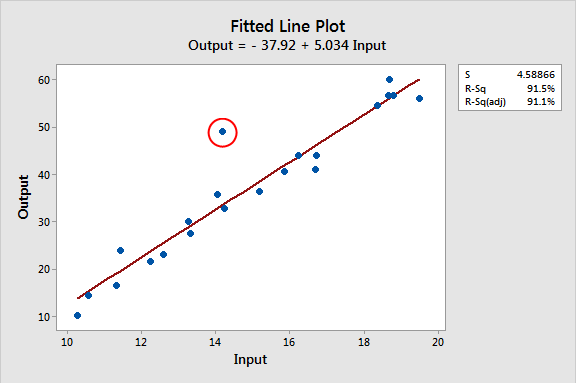
\includegraphics[width=0.55\linewidth]{images/Hình minh họa cho Outlier.png}
        \caption{Hình minh họa cho Outlier}
        \label{fig:placeholder}
    \end{figure}
\end{frame}
%%=====================================
\begin{frame}
\frametitle{Sự tác động của Outlier đến mô hình hồi quy}
	\begin{figure}
	    \centering
	    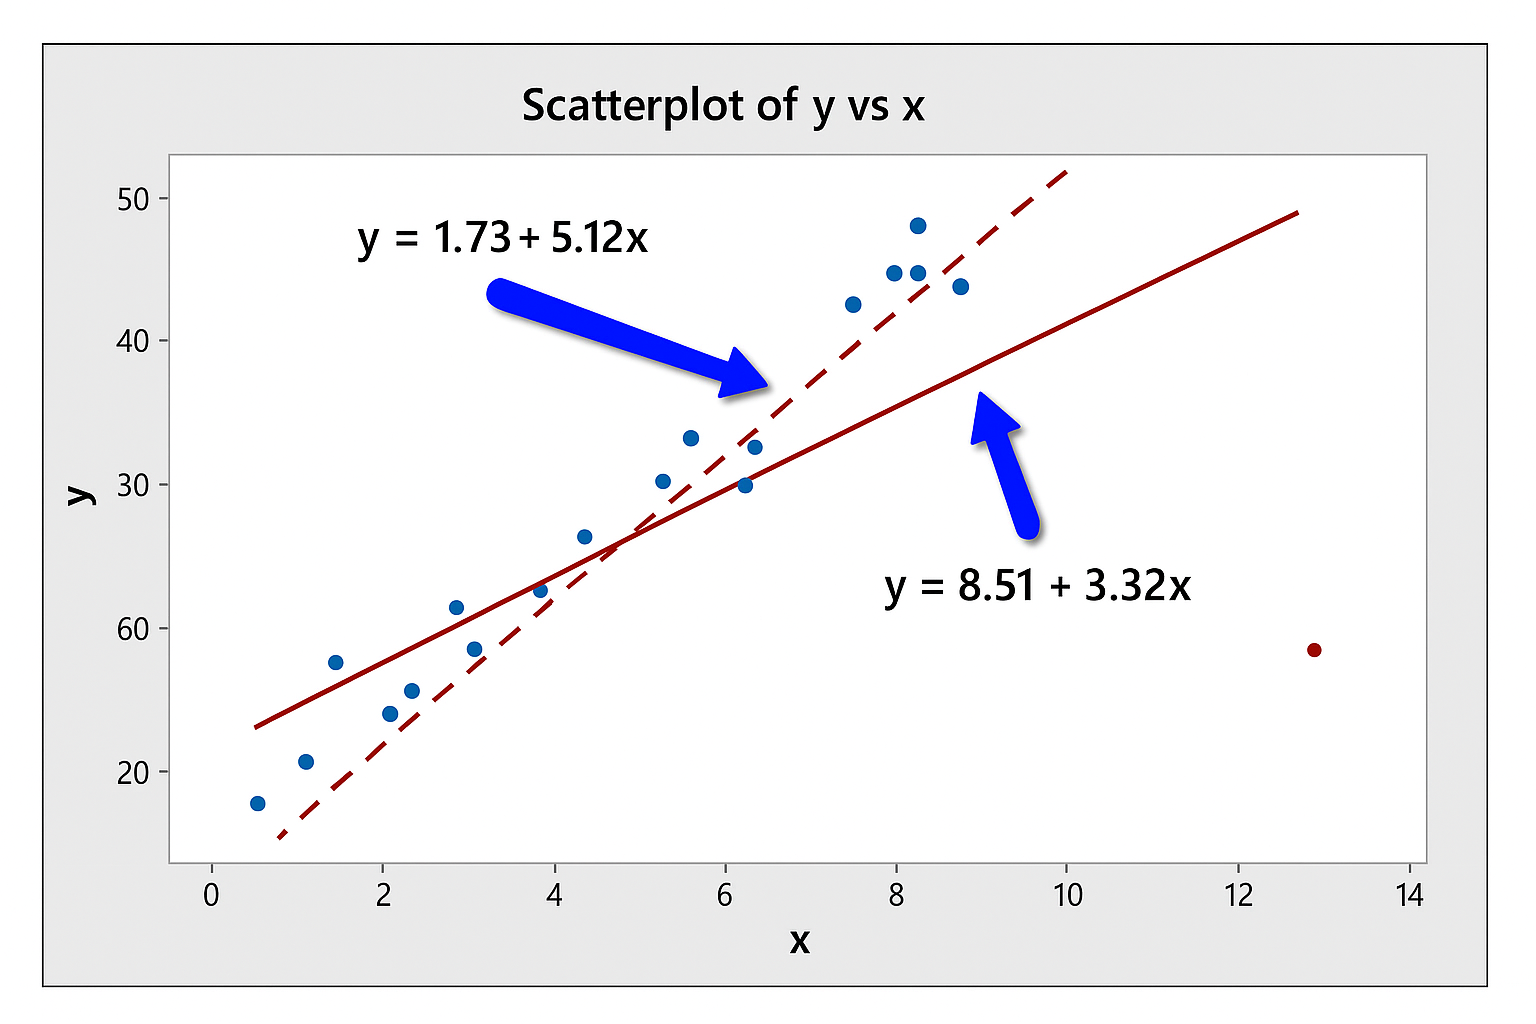
\includegraphics[width=0.6\linewidth]{images/Sự tác động của Outlier đến mô hình.png}
	    \caption{Sự tác động của Outlier đến mô hình}
	    \label{fig:placeholder}
	\end{figure}
    \begin{itemize}
        \item Đường nét liền thể hiện mô hình hồi quy tuyến tính khi giữ lại Outlier.
        \item Đường nét đứt thể hiện mô hình hồi quy tuyến tính khi đã loại bỏ Outlier.
    \end{itemize}
\end{frame}
\subsection{Độ đo Leverage}
\begin{frame}
\frametitle{Độ đo Leverage}
	\begin{itemize}
    \begin{block}{Định nghĩa}
    \textbf{Leverage} là độ đo khoảng cách giữa một điểm dữ liệu và phần còn lại của bộ dữ liệu dựa trên miền giá trị của bộ dữ liệu, được xác định bởi công thức:
    $$ h_{k j}=\frac{1}{n}+\frac{\left(z_{kj}-\overline{z}\right)^{2}}{\sum_{j=1}^{n}\left(z_{kj}-\overline{z}\right)^{2}}$$
    \end{block}
    \item Những điểm nằm xa so với bộ dữ liệu gọi là những điểm high leverage, ngược thì gọi là lower leverage.
    \item \textbf{Kết luận:} Ta thấy $h_{kj}$ luôn nằm giữa 1/n và 1. Hơn nữa, leverage trung bình cho các quan sát luôn bằng (p+1)/n, p là biến số dự đoán. Do vậy, nếu một quan sát mà có độ đo leverage quá lớn so với (p+1)/n ta có thể nghi ngờ là một điểm high leverage.
\end{itemize}
\end{frame}
%%=====================================
\begin{frame}
\frametitle{Nhận xét}
\begin{itemize}
   \item Càng có nhiều điểm dữ liệu nằm gần nhau thì sức ảnh hưởng hay độ lớn của điểm high leverage càng giảm.
   \item Các điểm high leverage có tác động rất lớn đến mô hình, điểm nào có giá trị của biến dự đoán nằm càng xa khỏi bộ dữ liệu thì tác động càng lớn.
   \item Những điểm $h_{kj} > 3*\overline{h}$ thì được coi là những outlier, với $\overline{h} = \dfrac{1}{n}\sum_{j=1}^n{h_{kj}}$
\end{itemize}
\end{frame}
%%=====================================
\begin{frame}
\frametitle{Ví dụ}

Để nghiên cứu sự phụ thuộc giữa điểm thi cuối kỳ $Y$ (tính theo thang 10) và số giờ tự học mỗi tuần $Z_1$, số giờ ngủ trung bình mỗi đêm $Z_2$ (đơn vị giờ), người ta điều tra ngẫu nhiên 12 sinh viên đại học của một trường, thu được bảng số liệu sau:

\resizebox{\textwidth}{!}{%
\begin{tabular}{|c|c|c|}
\hline 
$Y$ (Điểm thi cuối kỳ) & $Z_1$ (Số giờ tự học mỗi tuần) & $Z_2$ (Số giờ ngủ trung bình mỗi đêm) \\
\hline 
5.8 & 6.5 & 6.5 \\
6.5 & 7.0 & 6.0 \\
7.0 & 6.5 & 7.0 \\
7.5 & 8.0 & 6.5 \\
8.0 & 9.0 & 7.2 \\
8.2 & 10.0 & 6.8 \\
7.8 & 8.6 & 7.5 \\
8.8 & 11.0 & 7.0 \\
9.0 & 12.0 & 6.7 \\
6.0 & 6.0 & 6.0 \\
8.3 & 9.5 & 7.8 \\
9.2 & 2.0 & 5.5 \\
\hline
\end{tabular}%
}

\end{frame}

%%=====================================
\begin{frame}
\frametitle{Ví dụ}

Ta có bảng sau:

\resizebox{\textwidth}{!}{%
\begin{tabular}{|c|ccc|c|ccc|}
\hline 
$j$ & $z_1$ & $h_{1j}$ & $h_{1 j} > 3*\frac{1}{n}\sum_{j=1}^{n}{h_{1 j}}$ 
& $j$ & $z_2$ & $h_{2j}$ & $h_{2 j} > 3*\frac{1}{n}\sum_{j=1}^{n}{h_{2 j}}$ \\
\hline
1 & 6.5 & 0.1125 & 0 & 1 & 6.5 & 0.0924 & 0 \\
2 & 7.0 & 0.0964 & 0 & 2 & 6.0 & 0.1881 & 0 \\
3 & 6.5 & 0.1125 & 0 & 3 & 7.0 & 0.1011 & 0 \\
4 & 8.0 & 0.0833 & 0 & 4 & 6.5 & 0.0924 & 0 \\
5 & 9.0 & 0.0959 & 0 & 5 & 7.2 & 0.1338 & 0 \\
6 & 10.0 & 0.1341 & 0 & 6 & 6.8 & 0.0851 & 0 \\
7 & 8.6 & 0.0878 & 0 & 7 & 7.5 & 0.2142 & 0 \\
8 & 11.0 & 0.1979 & 0 & 8 & 7.0 & 0.1011 & 0 \\
9 & 12.0 & 0.2873 & 0 & 9 & 6.7 & 0.0833 & 0 \\
10 & 6.0 & 0.1350 & 0 & 10 & 6.0 & 0.1881 & 0 \\
11 & 9.5 & 0.1118 & 0 & 11 & 7.8 & 0.3322 & 0 \\
12 & 2.0 & 0.5455 & 1 & 12 & 5.5 & 4.7122 & 1 \\
\hline
\end{tabular}%
}

\vspace{0.5em}
Trong bộ dữ liệu ở ví dụ 6.1, quan sát thứ 12 ($Y=9.2$, $z_1 = 2.0$, $z_2 = 5.5$) là một \textbf{outlier} vì điểm này có kết quả thi rất cao mặc dù thời gian học và ngủ thấp, trái ngược với xu hướng chung.
\end{frame}

%%======================
%%=====================================
\subsection{Quy tắc 1.5IQR}
\begin{frame}
\frametitle{Quy tắc 1.5IQR}
\begin{itemize}
    \item Bất kì tập dữ liệu nào cũng có thể mô tả bằng năm giá trị đặc trưng, năm giá trị này cung cấp thông tin cần thiết để định vị outlier bao gồm (lần lượt theo thứ tự tăng dần).
    \begin{itemize}
        \item Giá trị nhỏ nhất hoặc thấp nhất của tập dữ liệu.
        \item Tứ phân vị thứ nhất $Q_1$: Phân vị mức 25\%.
        \item Tứ phân vị thứ hai $Q_2$: Phân vị mức 50\%.
        \item Tứ phân vị thứ ba $Q_3$: Phân vị mức 75\%.
        \item Giá trị lớn nhất hoặc cao nhất của tập dữ liệu.
    \end{itemize}
    \item \textbf{Khoảng cách tứ phân vị} là giá trị
    \[
    IQR = Q_3 - Q_1
    \]
    Khi đó nếu $x \notin \left[Q_1 - 1.5IQR, Q_3 + 1.5IQR\right]$ thì $x$ sẽ được coi là một điểm outlier.
\end{itemize}
\end{frame}
%%=====================================
%%=====================================
\begin{frame}
\frametitle{Ví dụ}
	    Một hệ thống ghi lại tốc độ (đơn vị: km/h) của 25 xe qua trạm như sau: 
        \begin{center}
            \begin{tabular}{|c|c|c|c|c|c|c|c|c|c|c|c|c|}
	\hline 
	20 & 41 & 41 & 80 & 40 & 52 & 52 & 52 & 60 & 55 & 60 & 60 & 62 \\ \hline
60 & 55 & 60 & 55 & 92 & 70 & 35 & 40 & 30 & 30 & 80 & 25 &  \\ \hline
\end{tabular}
        \end{center}
        Tìm các số liệu bất thường (nếu có) trong mẫu số liệu trên.
\end{frame}
%%=====================================
\begin{frame}
\frametitle{Ví dụ}
\begin{itemize}
	\item Sắp xếp dữ liệu theo thứ tự tăng dần: 20, 25, 30, 30, 35, 40, 40, 41, 41, 52, 52, 52, 55, 55,  60, 60, 60, 60, 60, 62, 70, 80, 80, 92.
    \item $Q_1$ là trung bình cộng giá trị thứ 6 và 7 nên $Q_1 = \dfrac{40 + 40}{2} = 40$.
    \item $Q_3$ là trung bình cộng giá trị thứ 19 và 20 nên $Q_3 = \dfrac{60 + 60}{2} = 60$.
    \item $IQR = Q_3 - Q_1 = 60 - 40 = 20$.
    \item Giới hạn dưới: $Lower = Q_1 - 1.5IQR = 40 - 1.5*20 = 40 - 30 = 10$.
    \item Giới hạn trên: $Upper = Q_3 + 1.5IQR = 60 + 1.5*20 = 60 + 30 =  90$.
\end{itemize}
\textbf{Kết luận}: Trong tập dữ liệu này, giá trị 92 là một outlier vì nó nằm ngoài khoảng $(Lower, Upper) = (10,90)$
\end{frame}
%%=====================================
\begin{frame}
\frametitle{Nhận xét}
Quy tắc \textit{1.5IQR} loại bỏ outlier được bắt nguồn từ quy tắc $3 \sigma$ trong lý thuyết xác suất. Quy tắc này phát biểu như sau:\textit{"Gần như chắc chắn rằng (với độ tin cậy khoảng 99,73\%) biến ngẫu nhiên $X$ có phân phối chuẩn} $\mathcal{N}(\mu, \sigma^2)$ \textit{sẽ lấy giá trị trong khoảng lân cận $3 \sigma$ của giá trị trung bình $\mu$"}. 
Với quy tắc này, ta có thể coi các giá trị nằm ngoài khoảng $(\mu - 3\sigma, \mu+3\sigma)$ là outlier. Tuy nghiên trên thực tế, khoảng $\left[Q_1-1.5IQR;Q_3+1.5IQR\right]$ chưa lấy được hết lân cận $3 \sigma$ mà chỉ lấy được tới lân cận $2.7 \sigma$ của giá trị trung bình $\mu$.
Do đó nếu cần thiết, ta có thể hiệu chỉnh quy tắc này trở thành quy tắc $1.7IQR$ để có thể lấy được hết lân cận, khi đó, nếu $x \notin \left[Q_1-1.7IQR; Q_3+1.7IQR\right]$ thì $x$ được coi là một điểm outlier.
\end{frame}
%%============================
\subsection{Giá trị $t-$statistic và $p-$value}
\begin{frame}
\frametitle{Định nghĩa $p-$value và $t-$statistic}
\begin{block}{Định nghĩa}
\begin{itemize}
   \item \textbf{$p-$value} là giá trị có ý nghĩa biên của một kiểm định giả thuyết thống kê, đại diện cho xác suất xảy ra một sự kiện cụ thể, dùng để đánh giá tính đáng tin cậy của một kết quả thống kê và quyết định liệu ta có đủ bằng chứng thống kê để bác bỏ giả thuyết không hay không.
   \item \textbf{$t-$statistic} là đại lượng kiểm định dùng để đánh giá xem một hệ số hồi quy $\beta_i$ có khác không một cách có ý nghĩa thống kê hay không, bằng cách chuẩn hóa $\widehat{\beta_i}$ theo độ lệch chuẩn của nó.
\end{itemize}
\end{block}
\end{frame}
%%=====================================
\begin{frame}
\frametitle{Tìm giá trị $t-$statistic và $p-$value}
   Xét cặp giả thuyết và đối thuyết sau với mỗi $i=\overline{1,r}$.
   \[
   H_0: \beta_i = 0, H_1: \beta_i \ne 0  
   \]
   Việc bác bỏ hay chấp nhận giả thuyết $H_0$ được thực hiện thông qua giá trị $t-$statistic được xác định bởi công thức:
       \[
       t-statistic(Z_i) = \dfrac{\widehat{\beta_i}}{\sqrt{\widehat{D}\left(\widehat{\beta_i}\right)}}
       \]
       Trong đó:
      \begin{itemize}
           \item $\widehat{\beta_i}$ là ước lượng hệ số hồi quy.
           \item $\widehat{D}\left(\widehat{\beta_i}\right)$ là phần tử thứ $i+1$ trên đường chéo chính của ma trận $\widehat{\sigma}^2\left(Z'Z\right)^{-1}$ với $\widehat{\sigma}^2 = \dfrac{1}{n-r-1}\sum_{j=1}^{n}{\widehat{\varepsilon_j}}^2$
       \end{itemize}
       
\end{frame}
%%=====================================
\begin{frame}
\frametitle{Tìm giá trị $t-$statistic và $p-$value}
Giá trị $p-$value là xác suất xảy ra sai lầm loại I (bác bỏ giả thuyết $H_0$ khi $H_0$ đúng)
\[
p-value \left(Z_i\right) = 2 \left(1-CDF(n,|t-statistic(Z_i|)\right)
\]
Trong đó: CDF là hàm phân phối xác suất của phân phối Student.
\end{frame}
%%=====================================
\begin{frame}
\begin{block}{Hệ quả}
\frametitle{Hệ quả}
\begin{itemize}
\item Nếu có mối quan hệ giữa $Z_i$ và $Y$, ta kỳ vọng $t-$statistic có phân phối Student với $n-r-1$ bậc tự do.
\item Giả thuyết $H_0: \beta_i = 0$ bị bác bỏ khi $p-$value < 5\% hoặc $p-$value < 1\% tùy mức ý nghĩa mà ta chọn (thường là 5\%)
\item Khi $ n \ge 30$, chúng lần lượt tương ứng với $t-$statistic $\ge 2$ hoặc $t-$statistic $\ge 2.75$.
\end{itemize}
\end{block}
\end{frame}
%%=====================================
\section{Kiểm định tính phụ thuộc vào biến của mô hình}
\subsection{Kiểm định F về ý nghĩa cùa mô hình hồi quy}
\begin{frame}
\frametitle{Kiểm định F về ý nghĩa của mô hình hồi quy}
Để kiểm định xem liệu trong số các biến $Z_1,Z_2,...,Z_k$ có biến nào là có thể loại khỏi mô hình hồi quy tuyến tính bội, ta tiến hành $F$-test. Việc này được tiến hành bằng cách giả sử rằng một vài hệ số $\beta_k$ của chúng ta bằng 0 (đồng nghĩa với việc loại bỏ $Z_k$) hay ta xét cặp giả thiết và đối thuyết như sau:
\begin{itemize}
    \item Giả thuyết $H_0$: $\beta_1$ =  $\beta_2$ = ... =  $\beta_k$ = 0
    \item Đối thuyết $H_1$: $\exists\beta_j \neq 0$ với j= $\overline{1,k}$ 
\end{itemize}

Tính toán đại lượng $F - score$:
\begin{equation*}
	F = \dfrac{(n-k-1)R^2}{k(1-R^2)}
\end{equation*}

Trong đó:
\[
R^{2} := 
\dfrac{\widehat{y}'\,\widehat{y} - n\bar{y}^{2}}
      {y'\,y - n\bar{y}^{2}}
= 
\dfrac{\displaystyle\sum_{i=1}^{n} (\widehat{y}_{i} - \bar{y})^{2}}
      {\displaystyle\sum_{i=1}^{n} (y_{i} - \bar{y})^{2}}
= 
1 - 
\dfrac{\displaystyle\sum_{i=1}^{n} \widehat{\varepsilon}_{i}^{2}}
      {\displaystyle\sum_{i=1}^{n} (y_{i} - \bar{y})^{2}}
\] 
\end{frame}
%%=====================================
\subsection{Các bước kiểm tra}
\begin{frame}
\frametitle{Các bước kiểm tra}
\begin{itemize}
 \item Bước 1: Tính đại lượng F-score.
    \item Bước 2: Tra bảng phân phối Fisher với bậc tự do là $k$ và $n-k-1$, mức ý nghĩa $\alpha$.
    \item Bước 3: Nếu $F > F_{k,n-k-1}(\alpha)$ thì ta bác bỏ $H_0$ và chấp nhận $H_1$.
\end{itemize}
\end{frame}
%%=====================================
\begin{frame}
\frametitle{Ví dụ}
 Để nghiên cứu sự phụ thuộc giữa doanh thu với chi phí sản xuất và chi phí tiếp thị (đơn vị Dollar), người ta điều
 tra ngẫu nhiên doanh thu của 12 công ty trong 12 thời kỳ, kết quả ta có bảng sau:
     {\scriptsize\begin{center}
            \begin{tabular}{|c|c|c|c|}
	\hline 
	STT & Y (Doanh thu) & $Z_1$ (Chi phí sản xuất) & $Z_2$ (Chi phí tiếp thị) \\
	\hline 
	1& 127 & 18 & 10 \\
      2&  149 & 25 & 11 \\
        3&106 & 19 &6\\
        4&163 & 24 &16\\
        5&102 & 15 &7\\
        6&180 &26 &17\\
        7&161 &25 &14\\
        8&128 &16 &12\\
        9&139 &17 &12\\
        10&144 &23 &12\\
        11&159 &22 &14\\
        12&138 &15 &15\\
	\hline
        
	   \end{tabular}
        \end{center}}
        Ta đi sẽ kiểm tra xem mô hình có phụ thuộc vào biến hay không với $\alpha = 0,05$.
\end{frame}
%%=====================================
\begin{frame}
\frametitle{Ví dụ}
Xét mô hình hồi quy tuyến tính cổ điển, ta có: 
\[
y_i = \beta_0 + \beta_1z_{j1} + \beta_2z_{j2} + \varepsilon_j (j=\overline{1,12}).
\]
Từ bảng trên ta có:\\
\[
Z = \begin{bmatrix}
1 & 18 & 10 \\
1 & 25 & 11 \\
1 & 19 & 6 \\
1 & 24 & 16 \\
1 & 15 & 7 \\
1 & 26 & 17 \\
1 & 25 & 14 \\
1 & 16 & 12 \\
1 & 17 & 12 \\
1 & 23 & 12 \\
1 & 22 & 14 \\
1 & 15 & 15
\end{bmatrix}, y = \begin{bmatrix}
    127 \\ 149 \\ 106 \\ 163\\ 102 \\ 180\\ 161\\128\\139\\144\\159\\138
\end{bmatrix}
\]
\end{frame}
%%=====================================
\begin{frame}
\frametitle{Ví dụ}
Bằng phương pháp ước lượng bình phương cực tiểu, ta tín hđược giá trị ước lượng của các hệ số hồi quy
 như sau:\\
 \[
 \widehat{\beta} = (Z'Z)^{-1}Z'y = \begin{bmatrix}
     \dfrac{1422007}{44056}\\[0,5cm] \dfrac{275981}{110140}\\[0,5cm] \dfrac{209649}{44056}
 \end{bmatrix}
 \]
 Từ đây ta tính được phương trình hồi quy tuyến tính mẫu là:
 \[
 \widehat{y} = \dfrac{1422007}{44056} + \dfrac{275981}{110140}z_1 + \dfrac{209649}{44056}z_2.
 \]
 Suy ra sai số ước lượng của mô hình hồi quy tuyến tính được tính như sau: 
 \[
 \widehat{\varepsilon} = y - Z\widehat{\beta}
 \]
\end{frame}
%%=====================================
\begin{frame}
\frametitle{Ví dụ}
Bảng tính các giá trị $\widehat{y_j}, \widehat{\varepsilon_j}$: 
\begin{center}
    \begin{tabular}{|c|c|c|c|}
    \hline 
    STT & $y_j$ & $\widehat{y_j}$ & $\widehat{\varepsilon_j}$ \\
    \hline 
    1  & 127 & 124.9673 & 2.0327 \\
    2  & 149 & 147.2661 & 1.7339 \\
    3  & 106 & 108.4383 & -2.4383 \\
    4  & 163 & 168.5539 & -5.5539 \\
    5  & 102 & 103.1741 & -1.1741 \\
    6  & 180 & 178.3240 & 1.6760 \\
    7  & 161 & 161.5422 & -0.5422 \\
    8  & 128 & 129.4732 & -1.4732 \\
    9  & 139 & 131.9790 & 7.0210 \\
    10 & 144 & 147.0134 & -3.0134 \\
    11 & 159 & 154.0250 & 4.9750 \\
    12 & 138 & 141.2436 & -3.2440 \\
    \hline
\end{tabular}
\end{center}
\end{frame}
%%=====================================
\begin{frame}
\frametitle{Ví dụ}
Ta có:
\[\widehat{\varepsilon_j}'\widehat{\varepsilon_j}=\sum\limits_{j = 1}^n{\widehat{\varepsilon_j}^2} = 144.23042;
\]
\[
\sum_{i=1}^{12}(y_i - \overline{y})^2 =  \sum_{i=1}^{12}\left(y_i - \dfrac{424}{3}\right)^2 = \dfrac{17774}{3}.
\] 
Vậy $R^2 = 1 - \dfrac{144.2304}{\dfrac{17774}{3}} = 0.9757$
$$F = \dfrac{0.9757 * (12-2-1)}{2*(1-0.9757)} = 180.6852$$
Tra bảng Fisher ta được: $$F_{2,9}(0.05)=4.2565$$
Ta thấy $F > F_{2,9}(0.05)$, do đó ta cần bác bỏ giả thiết rằng $\beta_1 = \cdots = \beta_k = 0$, tức là có sự phụ thuộc tuyến tính vào các biến độc lập.
\end{frame}
%%=====================================
\section{Kiểm tra tính đa cộng tuyến của các biến dự đoán}
\subsection{Đa cộng tuyến}
\begin{frame}
\frametitle{Đa cộng tuyến}
Sự đa cộng tuyến giữa các biến dự đoán ám chỉ trường hợp mà ở đó, hai hay nhiều biến dự đoán có sự ràng buộc với nhau. Hệ quả điển hình của hiện tượng này đó là các phần tử trên đường chéo chính của ma trận $(\textbf{Z}'\textbf{Z})^{-1}$ sẽ rất lớn, dẫn đến các ước lượng $\widehat{\beta}_i$ lớn theo và gây cản trở trong việc xác định độ "quan trọng" (significant) của các biến dự đoán.
\end{frame}
%%=====================================
\subsection{Cách nhận biết hiện tượng đa cộng tuyến}
\begin{frame}
\frametitle{Cách nhận biết hiện tượng đa cộng tuyến}
\begin{itemize}
    \item Một số phần tử trên đường chéo chính của ma trận $(\textbf{Z}'\textbf{Z})^{-1}$ tỏ ra rất lớn.
    \item Các hệ số tương quan tuyến tính mẫu của các cặp $Z_i,Z_j$ là $r_{ij} = s_{ij}/\sqrt{s_{jj}s_{ii}}$ tỏ ra lớn $(|r_{ij}|\geq 0,7$), trong đó:
    $$s_{ij} = \dfrac{1}{n - 1}\sum\limits_{k=1}^n{(z_{ki} - \overline{z_i})  \times (z_{kj} -\overline{z_j})}$$
\end{itemize}
\end{frame}
%%=====================================
\subsection{Cách khắc phục hiện tượng đa cộng tuyến}
\begin{frame}
\frametitle{Cách khắc phục hiện tượng đa cộng tuyến}
\begin{enumerate}
    \item Tính các hệ số tương quan mẫu $r_{ij}$.
	\item Đặt $r_{0i}$ là hệ số tương quan tuyến tính mẫu giữa $Y$ và $Z_i$, cụ thể là:
	$$r_{0i} = s_{0i}/\sqrt{s_{ii}s_{00}}$$
	Trong đó:
    \begin{itemize}
    \item $s_{00} = \dfrac{1}{n-1}\sum\limits_{j=1}^n{(y_j - \overline{y}) \times( y_j-\overline{y}) }$ ; \item $s_{0i} = \dfrac{1}{n-1}\sum\limits_{j=1}^n{(y_j - \overline{y}) \times( z_{ji}-\overline{z_i}) }$ \end{itemize}
	Khi đó, nếu thấy $|r_{ij}| \geq 0,7$ thì:
	\begin{itemize}
	    \item Ta loại biến $Z_i$ ra khỏi mô hình nếu $|r_{0i}| < |r_{0j}|$.
	    \item Ta loại biến $Z_j$ ra khỏi mô hình nếu $|r_{0i}| > |r_{0j}|$.
	\end{itemize} 
	\item Thực hiện hồi quy sau khi ma trận $Z$ đã loại bỏ biến $Z_i$ hay $Z_j$.
\end{enumerate}
\end{frame}
%%=====================================
\begin{frame}
\frametitle{Ví dụ}
    
\end{frame}
\end{footnotesize}


%%=============================================================
%%=============================================================
%% NỘI DUNG MỚI BẮT ĐẦU TỪ ĐÂY
%%=============================================================
%%=============================================================

% ===============================================================
\section{Khảo sát phần dư}
% ===============================================================

% --- Slide Giới thiệu Phần dư ---
\begin{frame}
    \frametitle{Khảo sát phần dư }
    \begin{block}{Phần dư (Residual) là gì?}
        Là sự khác biệt giữa giá trị thực tế và giá trị mô hình dự đoán.
        \[ \widehat{\varepsilon_i} = y_i - \widehat{y_i} \]
        Phần dư chứa đựng thông tin về những gì mô hình chưa giải thích được.
    \end{block}
    
    \textbf{Mục tiêu:} Kiểm tra xem các giả định cốt lõi của Hồi quy Tuyến tính có bị vi phạm hay không. Một mô hình tốt sẽ có phần dư phân tán hoàn toàn ngẫu nhiên.
\end{frame}

% --- Slide Các giả định ---
\begin{frame}
    \frametitle{Bốn giả định cốt lõi cần kiểm tra}
    \begin{itemize}
        \item<1-> \textbf{Tính tuyến tính (Linearity):} Mối quan hệ giữa X và Y có thực sự là đường thẳng?
        
        \item<2-> \textbf{Phương sai không đổi (Homoscedasticity):} Sai số có ổn định trên mọi khoảng giá trị dự đoán không?
        
        \item<3-> \textbf{Phân phối chuẩn của sai số (Normality):} Sai số có tuân theo phân phối chuẩn không? (Quan trọng cho suy diễn thống kê).
        
        \item<4-> \textbf{Tính độc lập của sai số (Independence):} Các sai số có độc lập với nhau không? (Cực kỳ quan trọng với dữ liệu chuỗi thời gian).
    \end{itemize}
\end{frame}

% --- Slide Phần dư Student hóa ---
\begin{frame}
    \frametitle{Phần dư Student hóa (Studentized Residuals)}
    \framesubtitle{Tại sao cần chuẩn hóa phần dư?}
    
    \begin{block}{Vấn đề với phần dư thô}
        Các phần dư thô $\widehat{\varepsilon}_i = y_i - \widehat{y}_i$ có \textbf{phương sai không đồng nhất}:
        \[
        Var(\widehat{\varepsilon}_i) = \sigma^2(1 - h_{ii})
        \]
        
        \begin{itemize}
            \item $h_{ii}$ là \textbf{leverage} (độ đòn bẩy) của quan sát thứ $i$\footnotemark
            \item Các quan sát có $h_{ii}$ khác nhau $\Rightarrow$ Phương sai khác nhau
            \item Không thể so sánh trực tiếp để phát hiện outlier
        \end{itemize}
    \end{block}
\end{frame}

\begin{frame}
    \frametitle{Phần dư Student hóa (Studentized Residuals)}
    \framesubtitle{Công thức và quy tắc sử dụng}
    
    \begin{block}{Giải pháp: Student hóa phần dư}
        Chuẩn hóa mỗi phần dư bằng cách chia cho độ lệch chuẩn của chính nó:
        \[
        r_i = \frac{\widehat{\varepsilon}_i}{\widehat{\sigma}\sqrt{1 - h_{ii}}}
        \]
        
        Trong đó:
        \begin{itemize}
            \item $\widehat{\varepsilon}_i$ = Phần dư thô của quan sát thứ $i$
            \item $\widehat{\sigma}$ = Ước lượng độ lệch chuẩn sai số (từ mô hình)
            \item $h_{ii}$ = Leverage của quan sát thứ $i$
        \end{itemize}
    \end{block}
\end{frame}

\begin{frame}
    \frametitle{Phần dư Student hóa (Studentized Residuals)}
    \framesubtitle{Công thức và quy tắc sử dụng}
    
    \textbf{Ưu điểm}
    \begin{itemize}
        \item $r_i$ có phương sai \textbf{xấp xỉ bằng 1}
        \item Có thể so sánh giữa các quan sát
        \item Tuân theo phân phối chuẩn (nếu giả định đúng)
    \end{itemize}

    \textbf{Quy tắc phát hiện outlier}
    \begin{itemize}
        \item $|r_i| \leq 2$: Bình thường
        \item $|r_i| > 2$: Đáng ngờ
        \item $|r_i| > 3$: Outlier nghiêm trọng
    \end{itemize}
\end{frame}

% ===============================================================
\section{Các cách kiểm tra}
% ===============================================================

% --- Slide Phần dư vs. Giá trị dự đoán ---
\begin{frame}
    \frametitle{Vẽ biểu đồ phần dư theo giá trị dự đoán}
    \framesubtitle{Biểu đồ chẩn đoán quan trọng nhất}
    
    \begin{columns}[T] % T = top align
        \begin{column}{0.5\textwidth}
            \textbf{Dấu hiệu xấu:}
            \begin{itemize}
                \item \textbf{Hình cái phễu:} Phương sai thay đổi .
            \end{itemize}
            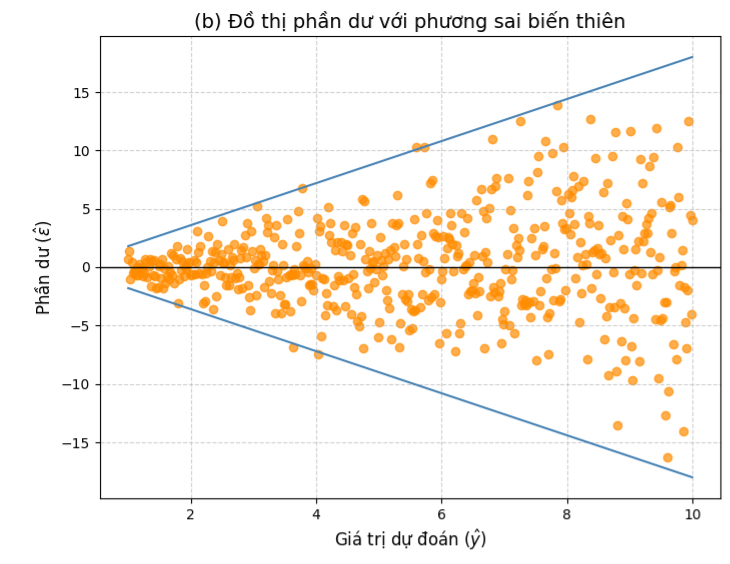
\includegraphics[width=0.9\linewidth]{images/b.png}
        \end{column}
        
        \begin{column}{0.5\textwidth}
            \textbf{Dấu hiệu tốt:}
            \begin{itemize}
                \item Phân tán ngẫu nhiên.
                \item Nằm trong một dải ngang.
            \end{itemize}
            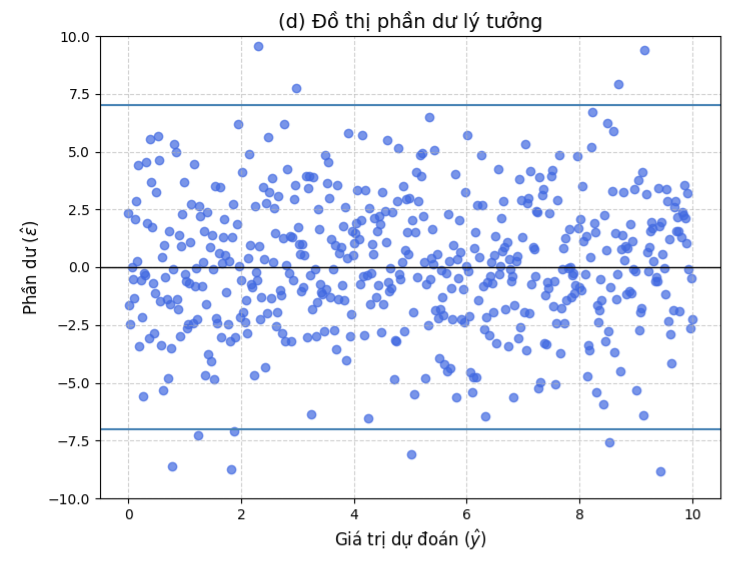
\includegraphics[width=0.9\linewidth]{images/d.png}
        \end{column}
    \end{columns}
\end{frame}

% --- Slide mới: Vẽ biểu đồ theo biến dự đoán ---
\begin{frame}
    \frametitle{Vẽ biểu đồ phần dư theo từng biến dự đoán ($X_i$)}
    \framesubtitle{Kiểm tra mối quan hệ phi tuyến bị bỏ sót}

    \begin{columns}[T] 
        \begin{column}{0.4\textwidth}
            \begin{itemize}
                \item \textbf{Hình parabol:} Bỏ sót quan hệ phi tuyến.
            \end{itemize}
            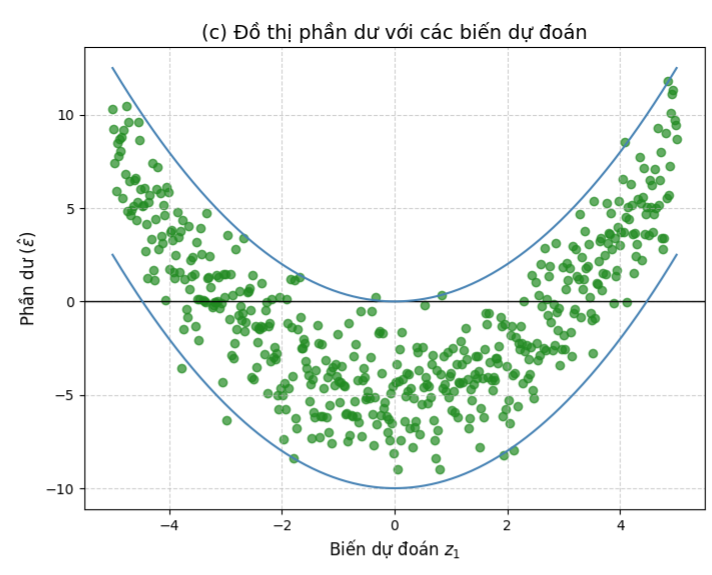
\includegraphics[width=0.9\linewidth]{images/c.png}
        \end{column}
        
        \begin{column}{0.6\textwidth}
            \begin{block}{Mục đích}
                Kiểm tra xem có một quy luật hệ thống nào giữa phần dư và một biến dự đoán \textbf{cụ thể} hay không.
            \end{block}
            
            \begin{alertblock}{Dấu hiệu vấn đề}
                Nếu biểu đồ cho thấy một quy luật có hệ thống, điều này gợi ý rằng mô hình cần có thêm các số hạng mới liên quan đến biến đó (ví dụ: $X_i^2$) để nắm bắt mối quan hệ phi tuyến.
            \end{alertblock}
        \end{column}
    \end{columns}
\end{frame}

% --- Slide Kiểm tra phân phối chuẩn ---
\begin{frame}
    \frametitle{Kiểm tra giả định phân phối chuẩn}
    \framesubtitle{Sử dụng Biểu đồ Q-Q và Histogram}
    
    \begin{block}{Tại sao quan trọng?}
        Các kiểm định t, F và khoảng tin cậy đều dựa trên giả định này. Nếu vi phạm, các giá trị p-value có thể không đáng tin cậy.
    \end{block}
    
    \begin{figure}
        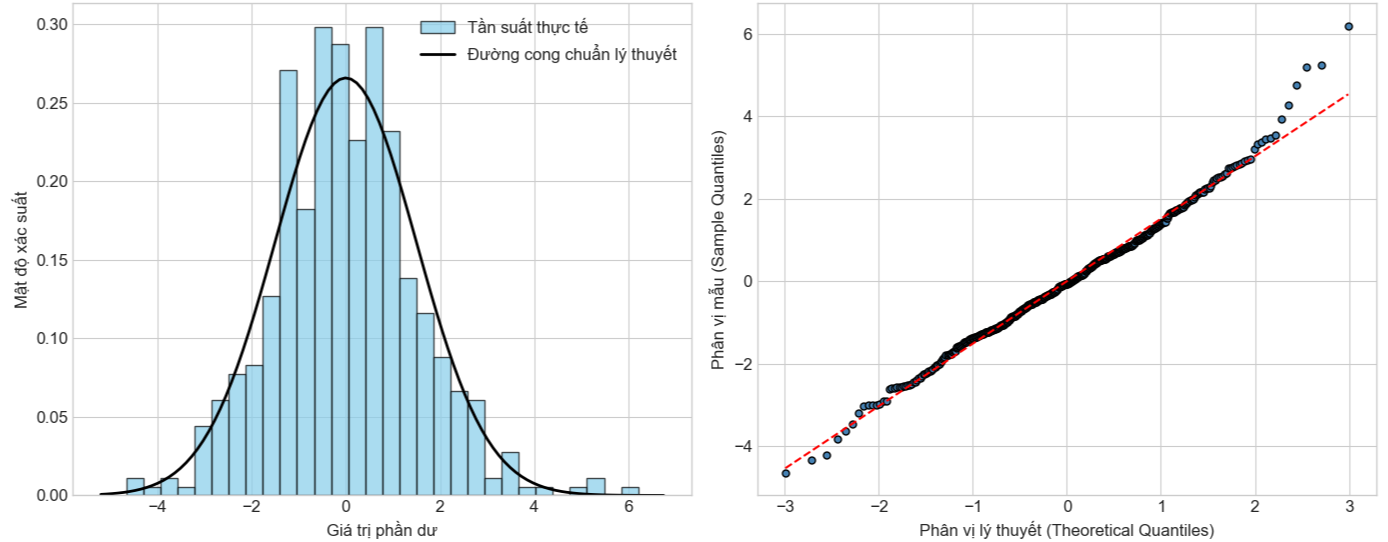
\includegraphics[width=0.7\linewidth]{images/Figure_1.png}
        \caption{Lý tưởng: Các điểm trên biểu đồ Q-Q nằm sát đường thẳng, và histogram có hình chuông.}
    \end{figure}
\end{frame}


% ===============================================================
\section{Kiểm định tính không tương quan của phần dư theo thời gian}
% ===============================================================

% --- Slide Kiểm định Tự tương quan ---
\begin{frame}
    \frametitle{Kiểm định Tự tương quan: Durbin-Watson}
    \framesubtitle{Đặc biệt quan trọng với dữ liệu chuỗi thời gian}

    Phổ biến nhất để kiểm tra tự tương quan \textbf{bậc một}, tức là mối liên hệ giữa $\varepsilon_t$ và $\varepsilon_{t-1}$.
    \begin{block}{Công thức Durbin-Watson}
        \[
        DW = \frac{\sum\limits_{t=2}^T(\widehat{\varepsilon}_t- \widehat{\varepsilon}_{t-1})^2}{\sum\limits_{t=1}^T(\widehat{\varepsilon}_t)^2} \quad \in [0, 4]
        \]
    \end{block}
    \begin{itemize}
        \item \textbf{Hạn chế:} Có "vùng không xác định" và không đáng tin cậy khi có biến trễ của Y.
    \end{itemize}
\end{frame}

\begin{frame}
    \frametitle{Kiểm định Tự tương quan: Durbin-Watson}
    \framesubtitle{Đặc biệt quan trọng với dữ liệu chuỗi thời gian}
    \textbf{Quy tắc quyết định:}
    
    Để đưa ra kết luận chính xác, cần so sánh giá trị DW với các giá trị tới hạn dL, dU từ bảng tra Durbin-Watson, dựa trên các yếu tố như mức ý nghĩa $\alpha$, cỡ mẫu n và số biến độc lập k. 
    \begin{itemize}
        \item $0 < DW < dL$ : Kết luận có tự tương quan dương.
        \item $dL \le DW \le dU$ : Không thể kết luận (vùng không xác định).
        \item $dU < DW < 4 - dU$ : Kết luận không có tự tương quan bậc nhất.
        \item $4 - dU \le DW \le 4 - dL$: Không thể kết luận.
        \item $4 - dL < DW < 4$: Kết luận có tự tương quan âm.
    \end{itemize}
\end{frame}

\begin{frame}
    \frametitle{Kiểm định Tự tương quan: Breusch-Godfrey}
    \framesubtitle{Kiểm định tổng quát cho tự tương quan bậc cao}

    Kiểm định Breusch-Godfrey (BG) là một kiểm định tổng quát và mạnh mẽ hơn DW, dùng để kiểm tra tự tương quan bậc cao.
    
    \textbf{Cách hoạt động:} Chạy một hồi quy phụ của phần dư theo các biến độc lập ban đầu và các phần dư trễ ($\varepsilon_{t-1},...,\varepsilon_{t-p})$.
    
    \begin{block}{Mô hình hồi quy phụ}
    \setlength{\abovedisplayskip}{0pt}
        \[
        \widehat{\varepsilon}_t = \alpha_0 + \beta_1 X_{1,t} + \ldots + \beta_k X_{k,t} + \alpha_1 \widehat{\varepsilon}_{t-1} + \alpha_2 \widehat{\varepsilon}_{t-2} + \ldots + \alpha_p \widehat{\varepsilon}_{t-p} + u_t
        \]
    \end{block}
    
    \begin{itemize}
        \item \textbf{Giả thuyết:} $H_0: \alpha_1 = \alpha_2 = \ldots = \alpha_p = 0$ (Không có tự tương quan đến bậc $p$).
        \item \textbf{Thống kê kiểm định:} $LM = nR^2 \sim \chi^2(p)$
        \item \textbf{Quyết định:} Nếu $p$-value của thống kê $LM$ là nhỏ ($< 0.05$), ta bác bỏ $H_0$ và kết luận có tồn tại tự tương quan.
    \end{itemize}
\end{frame}


% ===============================================================
\section{Xác định các biến quan trọng}
% ===============================================================

% --- Slide Tổng quan ---
\begin{frame}
    \frametitle{Xác định các biến quan trọng}
    \framesubtitle{Tại sao cần lựa chọn biến?}
    Vấn đề với mô hình có quá nhiều biến:
    \begin{itemize}
        \item \textbf{Overfitting:} Mô hình fit tốt trên train ($R^2$ cao) nhưng dự đoán kém trên test
        \item \textbf{Đa cộng tuyến:} Các hệ số không ổn định, phương sai lớn và p-value không đáng tin cậy.
        \item \textbf{Khó diễn giải:} Quá nhiều biến làm mô hình phức tạp
        \item \textbf{Chi phí thu thập dữ liệu:} Thực tế không cần thiết
    \end{itemize}
    \textbf{Mục tiêu:} Tìm tập con biến nhỏ nhất nhưng vẫn giải thích tốt biến phụ thuộc.
        
    \textit{"As simple as possible, but not simpler"} - Einstein
\end{frame}

% --- Slide Các phương pháp lựa chọn biến ---
\begin{frame}
    \frametitle{Các tiêu chí đánh giá mô hình}
    \framesubtitle{Hồi quy từng bước (Stepwise Regression)}
    Một thuật toán tự động để thêm/bớt các biến dựa trên một tiêu chí thống kê (ví dụ: F-test, p-value).
    
    \textbf{Lựa chọn tiến (Forward Selection):}
    \begin{enumerate}
        \item Bắt đầu với mô hình rỗng (chỉ có hệ số chặn).
        \item Lần lượt thêm từng biến vào và chọn biến có p-value thấp nhất (và < $\alpha$).
        \item Lặp lại cho đến khi không còn biến nào có thể thêm vào.
    \end{enumerate}
\end{frame}

\begin{frame}
    \frametitle{Các tiêu chí đánh giá mô hình}
    \framesubtitle{Hồi quy từng bước (Stepwise Regression)}

    \textbf{Loại bỏ lùi (Backward Elimination):}
    \begin{enumerate}
        \item Bắt đầu với mô hình đầy đủ (chứa tất cả các biến).
        \item Tìm biến có p-value cao nhất và lớn hơn ngưỡng $\alpha$ (thường là 0.05).
        \item \textbf{Loại bỏ} duy nhất biến đó.
        \item Chạy lại mô hình với các biến còn lại.
        \item Lặp lại quy trình cho đến khi tất cả các biến trong mô hình đều có p-value nhỏ hơn $\alpha$.
    \end{enumerate}
\end{frame}

\begin{frame}
    \frametitle{Các tiêu chí đánh giá mô hình}
    \framesubtitle{Hồi quy từng bước (Stepwise Regression)}
    
    \textbf{Chọn hỗn hợp (Mixed Selection):}
    \begin{itemize}
        \item Đây là phương pháp kết hợp cả Forward và Backward.
        \item Sau mỗi bước thêm vào một biến mới, thuật toán sẽ kiểm tra lại tất cả các biến đã có trong mô hình.
        \item Nếu có biến nào trở nên không còn ý nghĩa (ví dụ p-value > $\alpha$), biến đó sẽ bị loại ra.
        \item Quá trình dừng lại khi không thể thêm vào hay loại ra bất kỳ biến nào nữa.
    \end{itemize}
\end{frame}

\begin{frame}
    \frametitle{Các tiêu chí đánh giá mô hình}
    \framesubtitle{Hệ số xác định $R^2$ hiệu chỉnh}
    Hệ số xác định $R^2$:
    \[
    R^2 = 1 - \frac{RSS}{TSS} 
    \]
    $R^2$ hiệu chỉnh:
    \[
    R^2_{adj} = 1 - \frac{RSS}{TSS}.\frac{n-1}{n-p-1}
    \]
    \begin{itemize}
        \item $R^2$: Luôn tăng khi thêm biến (kể cả biến vô dụng)
        \item $R^2_{adj}$: Có thể giảm nếu biến thêm vào không đủ tốt
        \item \textbf{Quy tắc:} Chọn mô hình có $R^2_{adj}$ cao nhất
    \end{itemize}
\end{frame}

\begin{frame}
    \frametitle{Các tiêu chí đánh giá mô hình}
    \framesubtitle{Mallow's Cp}
    So sánh mô hình con với mô hình đầy đủ. Mô hình tốt sẽ có giá trị $C_p$ nhỏ và xấp xỉ số tham số ($p+1$).
    \[C_p = \frac{RSS_p}{\widehat{\sigma}^2} - n + 2(p+1)\]
    \begin{enumerate}
        \item Tính $C_p$ cho tất cả các mô hình con
        \item Vẽ đồ thị $C_p$ vs. $p+1$
        \item Chọn mô hình có $C_p$ \textbf{nhỏ} và các điểm $(p+1,C_p)$ nằm gần đường chéo $45^{\circ}$
    \end{enumerate}
\end{frame}

\begin{frame}
    \frametitle{Các tiêu chí đánh giá mô hình}
    \framesubtitle{AIC (Akaike's Information Criterion)}
    Mô hình có AIC nhỏ hơn thì tốt hơn.
    \[ AIC = n \ln(\frac{RSS_p}{n}) + 2(p+1) \]
    \textbf{Ưu điểm}
    \begin{itemize}
        \item Có xu hướng chọn mô hình tốt nhất để tối ưu hóa khả năng dự đoán 
        \item Thường hoạt động tốt với mẫu nhỏ
    \end{itemize}
    
    \textbf{Nhược điểm}
    \begin{itemize}
        \item Khi cỡ mẫu $n$ rất lớn, AIC vẫn có xác suất chọn phải mô hình quá phức tạp (overfitting) và không hội tụ về "mô hình thật" (true model).
    \end{itemize}
\end{frame}
\begin{frame}
    \frametitle{Các tiêu chí đánh giá mô hình}
    \framesubtitle{BIC (Bayesian Information Criterion)}
    Tương tự AIC nhưng phạt nặng hơn khi thêm biến (với n lớn)
    \[ BIC = n \ln\left(\frac{RSS_p}{n}\right) + (p+1)\ln(n) \]
    
    \textbf{Ưu điểm}
    \begin{itemize}
        \item Ưu tiên sự đơn giản: Mức phạt $\ln(n)$ rất nặng, giúp tránh overfitting hiệu quả trong các bộ dữ liệu lớn.
        \item Khi $n$ đủ lớn, BIC có khả năng tìm ra "mô hình thật" với xác suất cao (tốt cho mục tiêu giải thích).
    \end{itemize}
    
    \textbf{Nhược điểm}
    \begin{itemize}
        \item Không phù hợp với các bộ dữ liệu mẫu nhỏ, có xu hướng chọn mô hình quá đơn giản (under-fitting).
    \end{itemize}
\end{frame}


\begin{frame}
    \frametitle{So sánh các phương pháp lựa chọn biến}
    
    \begin{table}
    \centering
    \scriptsize
    \begin{tabular}{|l|c|c|l|}
    \hline
    \textbf{Phương pháp} & \textbf{Mục tiêu} & \textbf{Tốc độ} & \textbf{Ghi chú} \\
    \hline
    Stepwise & Minimize AIC / RSS & Trung bình & Tự động thêm hoặc loại biến \\
    \hline
    $R^2_{adj}$ & Maximize & Nhanh & Đơn giản, dễ so sánh mô hình \\
    \hline
    AIC & Minimize & Nhanh & Ưu tiên độ phù hợp (fit) \\
    \hline
    BIC & Minimize & Nhanh & Ưu tiên mô hình đơn giản \\
    \hline
    $C_p$ (Mallows) & $\approx p+1$ & Trung bình & Liên quan chặt chẽ với AIC \\
    \hline
    \end{tabular}
    \end{table}
\end{frame}


% ===============================================================
\section{Các bước thiết lập mô hình hồi quy tuyến tính}
% ===============================================================

% --- Slide Quy trình ---
\begin{frame}
    \frametitle{Quy trình 5 bước xây dựng mô hình hồi quy}
    \begin{enumerate}
        \item \textbf{Khám phá và Chuẩn bị dữ liệu (EDA):}
        \begin{itemize}
            \item Trực quan hóa, xử lý dữ liệu thiếu, kiểm tra đa cộng tuyến.
            \item Chia tập Train/Test ngay từ đầu
        \end{itemize}

        \item \textbf{Lựa chọn biến và Xây dựng mô hình (Trên tập Train):}
        \begin{itemize}
            \item Sử dụng Stepwise, p-value, AIC, Adjusted $R^2$, $C_p$ để chọn mô hình ứng viên.
        \end{itemize}

        \item \textbf{Chẩn đoán và Tinh chỉnh mô hình (Trên tập Train):}
        \begin{itemize}
            \item Kiểm tra giả định thông qua phần dư (tuyến tính, phương sai, chuẩn, độc lập).
            \item Phân tích outlier. Nếu vi phạm, quay lại Bước 2.
        \end{itemize}

        \item \textbf{Đánh giá hiệu năng cuối cùng (Trên tập Test):}
        \begin{itemize}
            \item Dùng mô hình cuối cùng để dự đoán trên tập test.
            \item Tính các chỉ số lỗi: MAPE, RMSE, MAE.
        \end{itemize}
        
        \item \textbf{Diễn giải và Báo cáo:}
        \begin{itemize}
            \item Trình bày phương trình, ý nghĩa hệ số và các kết quả đánh giá.
        \end{itemize}
    \end{enumerate}
\end{frame}
\input{chuong3/chuong3.tex}
\section{Xây dựng mô hình}
\begin{frame}
\frametitle{Xây dựng mô hình}
Ở các mục trước, chúng ta đã tìm hiểu về mô hình hồi quy tuyến tính đơn giản và mô hình hồi quy tuyến tính bội. 

Ở mục này, ta sẽ mở rộng mô hình bằng cách sử dụng nhiều hơn một biến phản hồi. 

Xét một mô hình gồm $m$ biến phản hồi $Y_1, Y_2, \dots, Y_m$ và $r$ biến dự đoán $Z_1, Z_2, \dots, Z_r$.  
Mỗi biến phản hồi $Y_j$ được giả thiết là một hàm tuyến tính của các biến dự đoán, ta viết:
\[
\begin{aligned}
Y_1 &= \beta_{01} + \beta_{11}Z_1 + \cdots + \beta_{r1}Z_r + \varepsilon_1 \\
Y_2 &= \beta_{02} + \beta_{12}Z_1 + \cdots + \beta_{r2}Z_r + \varepsilon_2 \\
&\vdots \\
Y_m &= \beta_{0m} + \beta_{1m}Z_1 + \cdots + \beta_{rm}Z_r + \varepsilon_m
\end{aligned}
\]
\end{frame}

%------------------------------------------------------------
\begin{frame}
\frametitle{Ký hiệu vector và ma trận}
Vector nhiễu $\boldsymbol{\varepsilon} = [\,\varepsilon_1 \ \varepsilon_2 \ \dots \ \varepsilon_m\,]'$ được giả sử tuân theo phân phối chuẩn m chiều với:
\[
E(\varepsilon) = 0, \quad Var(\varepsilon) = \Sigma
\]
trong đó $\Sigma$ là ma trận đối xứng xác định dương.

Để tiếp cận với công thức của mô hình hồi quy tuyến tính đa bội, ta ký hiệu:
\[
Y_j = [y_{j1} \ y_{j2} \ \dots \ y_{jm}]', \quad
Z_j = [z_{j0} \ z_{j1} \ \dots \ z_{jr}]', \quad
\varepsilon_{j} = [\varepsilon_{j1} \ \varepsilon_{j2} \ \dots \ \varepsilon_{jm}]'
\]
lần lượt là giá trị thu thập được của các biến phản hồi, biến dự đoán và nhiễu tại quan sát thứ j.
\end{frame}

%------------------------------------------------------------
\begin{frame} 
\frametitle{Dạng ma trận của mô hình} 
Để thuận tiện cho việc diễn đạt mô hình, các mô hình trên được viết lại dưới dạng ma trận. Khi đó ta có: 
\[ [Y] = \begin{bmatrix} y_{11} & y_{12} & \cdots & y_{1m} \\ y_{21} & y_{22} & \cdots & y_{2m} \\ \vdots & \vdots & \ddots & \vdots \\ y_{n1} & y_{n2} & \cdots & y_{nm} \end{bmatrix}_{n \times m}, 
\quad 
[\beta] = \begin{bmatrix} \beta_{01} & \beta_{02} & \cdots & \beta_{0m}\\ \beta_{11} & \beta_{12} & \cdots & \beta_{1m}\\ \vdots & \vdots & \ddots & \vdots\\ \beta_{r1} & \beta_{r2} & \cdots & \beta_{rm} \end{bmatrix}_{(r+1)\times m} \] 

\[ [\varepsilon] = \begin{bmatrix} \varepsilon_{11} & \varepsilon_{12} & \cdots & \varepsilon_{1m}\\ \varepsilon_{21} & \varepsilon_{22} & \cdots & \varepsilon_{2m}\\ \vdots & \vdots & \ddots & \vdots\\ \varepsilon_{n1} & \varepsilon_{n2} & \cdots & \varepsilon_{nm} \end{bmatrix}_{n \times m}, 
\quad 
Z = \begin{bmatrix} 1 & z_{11} & z_{12} & \cdots & z_{1r} \\ 1 & z_{21} & z_{22} & \cdots & z_{2r} \\ \vdots & \vdots & \vdots & \ddots & \vdots \\ 1 & z_{n1} & z_{n2} & \cdots & z_{nr} \end{bmatrix}_{n \times (r+1)} \] 
Từ các ma trận trên, mô hình hồi quy tuyến tính đa bội được viết gọn dưới dạng: 
\[
\begin{bmatrix}
Y
\end{bmatrix}_{n \times m}
=
Z_{n \times (r+1)}
\begin{bmatrix}
\beta
\end{bmatrix}_{(r+1) \times m}
+
\begin{bmatrix}
\varepsilon
\end{bmatrix}_{n \times m}
\]
\end{frame}

%------------------------------------------------------------
\begin{frame}
\frametitle{Các giả thiết của mô hình}
Các giả thiết của mô hình hồi quy tuyến tính đa biến:
\begin{itemize}
    \item $E(\boldsymbol{\varepsilon}_{(i)}) = 0$
    \item $\mathrm{Cov}(\boldsymbol{\varepsilon}_{(i)}, \boldsymbol{\varepsilon}_{(j)}) = \sigma_{ij} I, \quad \forall i,j = 1,\dots,m$
\end{itemize}
Ma trận hiệp phương sai của $m$ giá trị nhiễu tại cùng một quan sát $j$:
\[
\mathrm{Var}(\boldsymbol{\varepsilon}_j) = 
\boldsymbol{\Sigma} =
\begin{bmatrix}
\sigma_{11} & \sigma_{12} & \cdots & \sigma_{1m} \\
\sigma_{21} & \sigma_{22} & \cdots & \sigma_{2m} \\
\vdots & \vdots & \ddots & \vdots \\
\sigma_{m1} & \sigma_{m2} & \cdots & \sigma_{mm}
\end{bmatrix}, \quad \forall j = 1,\dots,n
\]
\textit{Như vậy, mô hình hồi quy tuyến tính đa bội là sự mở rộng tự nhiên của mô hình hồi quy tuyến tính bội, cho phép các biến phản hồi có thể tương quan với nhau.}
\end{frame}

%============================================================
\section{Ước lượng các tham số}
%------------------------------------------------------------
\subsection{Ước lượng bình phương cực tiểu của \texorpdfstring{$[\beta]$}{[beta]}}
%------------------------------------------------------------
\begin{frame}
\frametitle{Ước lượng bình phương cực tiểu của $[\beta]$}
Như đã đề cập ở phần trước, biến phản hồi thứ $j$ tuân theo mô hình hồi quy tuyến tính cổ điển:
\[
Y_{(j)} = Z\beta_{(j)} + \varepsilon_{(j)}
\]
Với mỗi mô hình như vậy, tổng bình phương nhiễu $RSS_j$ được cực tiểu hoá bởi:
\[
\widehat{\beta}_{(j)} = (Z'Z)^{-1}Z'Y_{(j)}
\]
Mặt khác, tổng bình phương nhiễu của toàn bộ mô hình hồi quy tuyến tính bội được cho bởi công thức:
\[
RSS([\beta]) = \sum_{j=1}^{n}RSS(\beta_{(j)}) 
= \sum_{j=1}^{n}(Y_{(j)} - Z\beta_{(j)})'(Y_{(j)} - Z\beta_{(j)})
\]
\end{frame}

%------------------------------------------------------------
\begin{frame}
\frametitle{Ước lượng bình phương cực tiểu của $[\beta]$}
Vì mỗi số hạng trong chuỗi tổng trên là không âm nên $RSS([\beta])$ của toàn bộ mô hình đạt cực tiểu khi từng $RSS(\beta_{(j)})$ đạt cực tiểu.  
Do đó:
\[
[\widehat{\boldsymbol{\beta}}]
=
\left[
\begin{array}{c: c: c: c}
\widehat{\boldsymbol{\beta}}_{(1)} & 
\widehat{\boldsymbol{\beta}}_{(2)} &
\cdots &
\widehat{\boldsymbol{\beta}}_{(m)}
\end{array}
\right]
=
(Z'Z)^{-1}Z'
\left[
\begin{array}{c: c: c: c}
Y_{(1)} &
Y_{(2)} &
\cdots &
Y_{(m)}
\end{array}
\right]
\]
\[
\boxed{
\widehat{[\beta]} = (Z'Z)^{-1}Z'[Y]
}
\]
\begin{block}{Kết luận}
$\widehat{[\beta]}$ là một \textbf{ước lượng bình phương cực tiểu} cho ma trận hệ số hồi quy $[\beta]$.
\end{block}
\end{frame}

%------------------------------------------------------------
\subsection{Ước lượng cho \texorpdfstring{$[Y]$, $[\varepsilon]$ và $\Sigma$}{[Y], [epsilon] và Σ}}
%------------------------------------------------------------
\begin{frame}
\frametitle{Ước lượng cho $[Y]$, $[\varepsilon]$ và $\Sigma$}
Sử dụng ước lượng bình phương cực tiểu $\widehat{[\beta]}$, ta có thể xác định các ma trận ước lượng sau:
\[
\widehat{[Y]} = Z\widehat{[\beta]} 
= Z(Z'Z)^{-1}Z'[Y]
\]
\[
\widehat{[\varepsilon]} = [Y] - \widehat{[Y]} 
= (I - Z(Z'Z)^{-1}Z')[Y]
\]
\begin{block}{Tính chất trực giao}
\[
Z'[\widehat{\varepsilon}] = Z'(I - Z(Z'Z)^{-1}Z')[Y] 
= (Z' - Z'Z(Z'Z)^{-1}Z')[Y] = 0
\]
\[
[\widehat{Y}]'[\widehat{\varepsilon}]
= (Z[\widehat{\beta}])'[\widehat{\varepsilon}]
= [\widehat{\beta}]'Z'[\widehat{\varepsilon}]
= 0
\]
\end{block}
Do đó mọi cột của $Z$ và $[\widehat{Y}]$ đều trực giao với mọi cột của $\widehat{[\varepsilon]}$.  

\end{frame}

%------------------------------------------------------------
\begin{frame}
\frametitle{Quan hệ giữa $[Y]'[Y]$, $\widehat{[Y]}'\widehat{[Y]}$ và $\widehat{[\varepsilon]}'\widehat{[\varepsilon]}$}
Từ đẳng thức $[Y] = \widehat{[Y]} + \widehat{[\varepsilon]}$ và tính trực giao ở trên, ta có:
\[
[Y]'[Y] = \widehat{[Y]}'\widehat{[Y]} + \widehat{[\varepsilon]}'\widehat{[\varepsilon]}
\]
\begin{block}{Kết luận}
\begin{center}
Tích vô hướng của vector phản hồi 

= Tích vô hướng của vector dự đoán + Tích vô hướng của vector nhiễu.
\end{center}
\end{block}
Ta sẽ sử dụng kết quả này để ước lượng ma trận hiệp phương sai $\Sigma$.
\end{frame}

%------------------------------------------------------------
\begin{frame}
\frametitle{Ước lượng hợp lý cực đại của $\Sigma$}

\begin{block}{Định lý 1}
Xét mô hình hồi quy tuyến tính bội:
\[
[Y] = Z[\beta] + [\varepsilon]
\]
với $\mathrm{rank}(Z)=r+1\le n-m$ và nhiễu $[\varepsilon]$ có phân phối chuẩn.  
Khi đó:
\[
\boxed{
\widehat{\Sigma} = \frac{1}{n}\widehat{[\varepsilon]}'\widehat{[\varepsilon]}
= \frac{1}{n}([Y] - Z\widehat{[\beta]})'([Y] - Z\widehat{[\beta]})
}
\]
là \textbf{ước lượng hợp lý cực đại} của ma trận hiệp phương sai $\Sigma$.
\end{block}
\textbf{Chứng minh.} Theo giả thiết, ta có $n$ quan sát và tại quan sát thứ $i$, vector nhiễu:
\[
\varepsilon_i = [\varepsilon_{i1} \ \varepsilon_{i2} \ \dots \ \varepsilon_{im}]
\sim \mathcal{N}_m(0, \Sigma)
\]
với hàm mật độ xác suất đồng thời:
{\tiny\[
f(\varepsilon_i)
= \frac{1}{\sqrt{(2\pi)^m \det \Sigma}}
\exp\!\left(-\frac{1}{2}\varepsilon_i \Sigma^{-1} \varepsilon_i'\right)
= \frac{1}{\sqrt{(2\pi)^m \det \Sigma}}
\exp\!\left(-\frac{1}{2}(Y_i - Z\beta_i)\Sigma^{-1}(Y_i - Z\beta_i)'\right)
\]}
\end{frame}

%------------------------------------------------------------
\begin{frame}
\frametitle{Ước lượng hợp lý cực đại của $\Sigma$}
Từ đó, hàm hợp lý cho toàn bộ $n$ quan sát là:
{\scriptsize
\[
\mathcal{L}([\beta], \Sigma, [Y])
= \prod_{i=1}^{n} f(\varepsilon_i)
= \frac{1}{\sqrt{(2\pi)^{mn}(\det \Sigma)^{n}}}
\exp\!\left(
-\frac{1}{2}
\sum_{i=1}^{n}
(Y_i - Z\beta_i)\Sigma^{-1}(Y_i - Z\beta_i)'
\right)
\]}
Đặt:
\[
Q = [q_{ij}]_{n\times n}
:= [\widehat{\varepsilon}]'[\widehat{\varepsilon}]
= ([Y] - Z[\widehat{\beta}])'([Y] - Z[\widehat{\beta}])
, \quad
q_{ij} = \sum_{k=1}^{n} (y_{ki} - \widehat{y}_{ki})(y_{kj} - \widehat{y}_{kj})
\]
Khi đó:
\[
\sum_{i=1}^{n} (Y_i - Z\beta_i)\Sigma^{-1}(Y_i - Z\beta_i)'
= \sum_{i=1}^{n} \left( \sum_{j=1}^{m} \sum_{k=1}^{m}
(y_{ij} - \widehat{y}_{ij})(\Sigma^{-1})_{jk}(y_{ik} - \widehat{y}_{ik}) \right)
\]
\[
= \sum_{j=1}^{m} \sum_{k=1}^{m}\left(  (\Sigma^{-1})_{jk}
\sum_{i=1}^{n} (y_{ij} - \widehat{y}_{ij})(y_{ik} - \widehat{y}_{ik}) \right)
= \sum_{j=1}^{m} \sum_{k=1}^{m} (\Sigma^{-1})_{jk} q_{jk}
= \mathrm{tr}(\Sigma^{-1} Q)
\]
\end{frame}

%------------------------------------------------------------
\begin{frame}
\frametitle{Ước lượng hợp lý cực đại của $\Sigma$}
Như vậy hàm hợp lý có thể được viết lại thành:
\[
\boxed{
\mathcal{L}([\beta],\Sigma,[Y]) =
\frac{1}{\sqrt{(2\pi)^{mn}(\det\Sigma)^{n}}}
\exp\!\left(-\frac{1}{2}\mathrm{tr}(\Sigma^{-1}Q)\right)
}
\]
Lấy log của hàm hợp lý:
\[
\log\mathcal{L}([\beta],\Sigma,[Y]) 
= -mn\log(2\pi) +n\log(\det\Sigma^{-1}) 
- \frac{1}{2}\mathrm{tr}(\Sigma^{-1}Q)
\]
Để cực đại hoá theo $\Sigma$, ta giải điều kiện đạo hàm bằng 0:
\[
\frac{\partial\log\mathcal{L}}{\partial\Sigma^{-1}} 
= \frac{n}{2}\Sigma - \frac{1}{2}Q = 0
\Rightarrow
\widehat{\Sigma} = \frac{Q}{n}
\]
\[
\boxed{
\widehat{\Sigma} = \frac{1}{n}([Y]-Z\widehat{[\beta]})'([Y]-Z\widehat{[\beta]})
}
\]
\end{frame}

%------------------------------------------------------------
\begin{frame}
\frametitle{Giá trị lớn nhất của hàm hợp lý}
\begin{block}{Hệ quả 1}
Giá trị lớn nhất của hàm hợp lý cực đại đạt tại $\widehat{[\beta]}$ và $\widehat{\Sigma}$ là:
\[
\mathcal{L}([\widehat{\beta}], \widehat{\Sigma}, [Y])
= \frac{1}{\sqrt{(2\pi)^{mn} (\det \Sigma)^{n}}}
\exp\!\left(-\frac{1}{2}\mathrm{tr}(\Sigma^{-1} Q)\right)
\]
\[
= \frac{1}{\sqrt{(2\pi)^{mn} (\det \Sigma)^{n}}}
\exp\!\left(-\frac{1}{2}\mathrm{tr}\!\left(n([\varepsilon]'[\varepsilon])^{-1}([\varepsilon]'[\varepsilon])\right)\right)
\]
\[
= \frac{1}{\sqrt{(2\pi)^{mn} (\det \Sigma)^{n}}}
\exp\!\left(-\frac{1}{2}\mathrm{tr}(nI)\right)
\]
\[
= (\det \Sigma)^{-n/2}(2\pi e)^{-mn/2}
\]
\end{block}
\textbf{Ghi chú:} Với ước lượng như trên, đại lượng $n\widehat{\Sigma}$ tuân theo phân phối $W_{p,\,n-r-1}(\Sigma)$ (phân phối Wishart).
\end{frame}

%============================================================
\section{Các tính chất quan trọng}
%============================================================
\begin{frame}{Ước lượng không chệch của $[\beta]$}
\begin{block}{Tính chất 1}
\[
\boxed{
\widehat{[\beta]} \text{ là ước lượng không chệch của } [\beta]
}
\]
\end{block}

Để chứng minh tính chất này, ta cần chỉ ra rằng:
\[
E(\widehat{[\beta]}) = [\beta]
\]
Thật vậy:
\[
\begin{aligned}
E(\widehat{[\beta]})
&= E\big((Z'Z)^{-1}Z'[Y]\big) \\
&= E\big((Z'Z)^{-1}Z'(Z[\beta] + [\varepsilon])\big) \\
&= E\big((Z'Z)^{-1}Z'Z[\beta]\big) + E\big((Z'Z)^{-1}Z'[\varepsilon]\big) \\
&= [\beta] + (Z'Z)^{-1}Z'E([\varepsilon]) \\
&= [\beta] + (Z'Z)^{-1}Z' \times 0 \\
&= [\beta]
\end{aligned}
\]
\textbf{Vậy } $\widehat{[\beta]}$ là ước lượng không chệch của $[\beta]$.
\end{frame}

%------------------------------------------------------------
\begin{frame}
\frametitle{Ước lượng hợp lý cực đại của $[\beta]$}
\begin{block}{Tính chất 2}
\[
\boxed{
\widehat{[\beta]} \text{ là ước lượng hợp lý cực đại của } [\beta]
} \quad \textit{(khi nhiễu $[\varepsilon]$ có phân phối chuẩn)}
\]
\end{block}

\textbf{Chứng minh.}  
Giả sử $[\varepsilon]$ có phân phối chuẩn thì hàm hợp lý của $n$ quan sát là:
{\scriptsize\[
\mathcal{L}([\beta], \Sigma, [Y])
= \prod_{i=1}^{n} f(\varepsilon_i)
= \frac{1}{\sqrt{(2\pi)^{mn} (\det \Sigma)^{n}}}
\exp\!\left(
-\frac{1}{2} \sum_{i=1}^{n} (Y_i - Z\beta_i)\Sigma^{-1}(Y_i - Z\beta_i)'
\right)
\]}
Đặt:
\[
S_i := (Y_i - Z\beta_i)\Sigma^{-1}(Y_i - Z\beta_i)'
\]

\[
S := \sum_{i=1}^{n}(Y_i - Z\beta_i)\Sigma^{-1}(Y_i - Z\beta_i)'
= \sum_{i=1}^{n} S_i
\]
\end{frame}

%------------------------------------------------------------
\begin{frame}
\frametitle{Ước lượng hợp lý cực đại của $[\beta]$}
Cực đại hóa $\mathcal{L}$ tương đương với cực tiểu hóa $S$.  
Lấy đạo hàm riêng:
\[
\frac{\partial S_i}{\partial [\beta]'}
= (\Sigma^{-1} + (\Sigma^{-1})')(Y_i' - [\beta]'Z_i')(-Z_i)
= -2\Sigma^{-1}(Y_i'Z_i - [\beta]'Z_i'Z_i)
\]
Xét đạo hàm bằng 0, lấy tổng từ $i=1$ đến $n$, ta được:
\[
\sum_{i=1}^{n}Y_i'Z_i = \sum_{i=1}^{n}[\beta]'(Z_i'Z_i)
\Rightarrow [Y]'Z = [\beta]'(Z'Z)
\]
\[
\boxed{\Rightarrow\widehat{[\beta]} = (Z'Z)^{-1}Z'[Y]}
\]
\textbf{Vậy } $\widehat{[\beta]}$ là ước lượng hợp lý cực đại của $[\beta]$.
\end{frame}

%------------------------------------------------------------
\begin{frame}
\frametitle{Kỳ vọng và hiệp phương sai}
\begin{block}{Tính chất 3}
\[
E([\widehat{\varepsilon}]) = 0, 
\quad
Cov(\beta_{(i)}, \beta_{(j)}) = \sigma_{ij}(Z'Z)^{-1}
\]
\end{block}
\textbf{Chứng minh.}
\[
E(\widehat{\varepsilon}_{(j)})
= E(Y_{(j)} - Z\widehat{\beta}_{(j)})
= E\big(Z(\beta_{(j)} - \widehat{\beta}_{(j)}) + \varepsilon_{(j)}\big)
= 0
\]
Đặt $C = (Z'Z)^{-1}Z'$, ta có:
\[
\begin{aligned}
\mathrm{Cov}(\widehat{\beta}_{(i)}, \widehat{\beta}_{(j)})
&= \mathrm{Cov}(CY_{(i)}, CY_{(j)})
= E\!\left(CY_{(i)} - E(CY_{(i)})\right)\!\left(CY_{(j)} - E(CY_{(j)})\right)' \\
&= C\,E\!\left((Y_{(i)} - Z\beta_{(i)})(Y_{(j)} - Z\beta_{(j)})'\right)C'
= C\,E(\varepsilon_{(i)}\varepsilon_{(j)}')\,C' \\
&= C\,\mathrm{Cov}(\varepsilon_{(i)}, \varepsilon_{(j)})\,C' = (Z'Z)^{-1}Z'(\sigma_{ij}I)Z(Z'Z)^{-1} \\
&= \sigma_{ij}(Z'Z)^{-1}
\end{aligned}
\]
\end{frame}

%------------------------------------------------------------
\begin{frame}
\frametitle{Phân phối của $\widehat{[\beta]}$}
\begin{block}{Tính chất 4}
\[
\boxed{
\widehat{[\beta]} \text{ có phân phối chuẩn.}
}
\]
\end{block}
\textbf{Chứng minh.}
Với giả thiết $\varepsilon_{(i)} \sim \mathcal{N}_n(0, \sigma_{ii}I)$, ta có:
\[
Y_{(i)} \sim \mathcal{N}_n(Z\beta, \sigma_{ii}I)
\Rightarrow 
\widehat{\beta}_{(i)} = (Z'Z)^{-1}ZY_{(i)} 
\sim \mathcal{N}_{r+1}\big(\beta_{(i)}, \sigma_{ii}(Z'Z)^{-1}\big)
\]
\textbf{Vậy } $\widehat{[\beta]}$ có phân phối chuẩn.
\end{frame}

%------------------------------------------------------------
\begin{frame}
\frametitle{Tính chệch của $\widehat{\Sigma}$}
\begin{block}{Tính chất 5}
\[
\boxed{
\widehat{\Sigma} \text{ là ước lượng chệch của } \Sigma
}
\]
\end{block}
\textbf{Chứng minh.}  
Ta cần chứng minh rằng:
\[
E(\widehat{\varepsilon}_{(i)}'\widehat{\varepsilon}_{(j)}) = \sigma_{ij}(n - r - 1)
\]
Đặt:
\[
H := Z(Z'Z)^{-1}Z', \quad I - H \text{ là ma trận dự đoán phần dư.}
\]
\[
E(\widehat{\varepsilon}_{(j)}'\widehat{\varepsilon}_{(k)}) 
= E([Y_{(j)} - \widehat{Y}_{(j)}]'[Y_{(k)} - \widehat{Y}_{(k)}])
= E([Y_{(j)}'(I-H)[Y_{(k)}])
\]
\[
= E(\varepsilon_{(j)}'(I-H)\varepsilon_{(k)}))
= \sigma_{jk}(n - r - 1)
\]
Suy ra:
\[
E(\widehat{\Sigma}) = \frac{n-r-1}{n}\Sigma
\Rightarrow \widehat{\Sigma} \text{ là ước lượng chệch của } \Sigma.
\]
\end{frame}

%------------------------------------------------------------
\begin{frame}
\frametitle{Ước lượng không chệch của $\Sigma$}
\begin{block}{Hệ quả 2}
\[
\boxed{
\widehat{\Sigma}^* = \frac{n}{n - r - 1}\widehat{\Sigma}
= \frac{n}{n - r - 1}\widehat{[\varepsilon]}'\widehat{[\varepsilon]}
}
\]
\textbf{là ước lượng không chệch của} $\Sigma$.
\end{block}
Khi đó:
\[
E(\widehat{\Sigma}^*) = \Sigma
\]
Như vậy, $\widehat{\Sigma}^*$ được dùng trong các kiểm định thống kê để đảm bảo tính không chệch.
\end{frame}

%============================================================
\section{Kiểm định tỷ số hợp lý cho tham số hồi quy}
%============================================================
\subsection{Kiểm định tỷ số hợp lý cho tham số hồi quy}
%------------------------------------------------------------
\begin{frame}
\frametitle{Kiểm định tỷ số hợp lý cho tham số hồi quy}
Tương tự như mục 6, ta tiến hành kiểm định xem liệu các biến phản hồi có tuân theo quy luật tuyến tính với toàn bộ biến phụ thuộc hay không.

Qua kiểm định, có thể \textbf{đơn giản hóa mô hình} mà không gây ra ảnh hưởng quá lớn tới độ hiệu quả.

Xét mô hình hồi quy tuyến tính đa bội:
\[
[Y] = Z[\beta] + [\varepsilon], \quad \text{với } \mathrm{rank}(Z) = r + 1 \le n - m.
\]
Tách $Z$ và $[\beta]$ thành hai phần:
\[
[Y] = Z[\beta] + [\varepsilon]
= \begin{bmatrix} Z_{(1)} & Z_{(2)} \end{bmatrix}
\begin{bmatrix} [\beta]_{(1)} \\ [\beta]_{(2)} \end{bmatrix} + [\varepsilon]
\]
Xét cặp giả thuyết và đối thuyết:
\[
\boxed{
H_0 : [\beta]_{(2)} = 0
\quad \text{và} \quad
H_1 : [\beta]_{(2)} \neq 0
}
\]
Dưới $H_0$, mô hình rút gọn trở thành:
\[
Y = Z_{(1)}[\beta]_{(1)} + [\varepsilon]_{(1)}
\]
\end{frame}

%------------------------------------------------------------
\begin{frame}
\frametitle{Kiểm định tỷ số hợp lý cho tham số hồi quy}
Độ lệch giữa các giá trị sai số trung bình bình phương hai mô hình được thể hiện qua:
\[
(\widehat{Y}_{(1)} - Z_{(1)}\widehat{[\beta]}_{(1)})'(\widehat{Y}_{(1)} - Z_{(1)}\widehat{[\beta]}_{(1)})
- (\widehat{Y} - Z\widehat{[\beta]})'(\widehat{Y} - Z\widehat{[\beta]})
= n(\widehat{\Sigma}_1 - \widehat{\Sigma})
\]
trong đó:
\[
\widehat{[\beta]}_{(1)} = (Z_{(1)}'Z_{(1)})^{-1}Z_{(1)}'[Y], 
\qquad 
\widehat{\Sigma}_1 = \frac{1}{n}(\widehat{Y}_{(1)} - Z_{(1)}\widehat{[\beta]}_{(1)})'(\widehat{Y}_{(1)} - Z_{(1)}\widehat{[\beta]}_{(1)})
\]
Xét tỷ số kiểm định $\Lambda$ được định nghĩa bởi:
\[
\Lambda = 
\frac{\max_{[\beta]_{(1)}, \Sigma} \mathcal{L}([\beta]_{(1)}, \Sigma)}
{\max_{[\beta], \Sigma} \mathcal{L}([\beta], \Sigma)}
= \frac{\mathcal{L}(\widehat{[\beta]}_{(1)}, \widehat{\Sigma}_1)}{\mathcal{L}(\widehat{[\beta]}, \widehat{\Sigma})}
= \left(\frac{\det \widehat{\Sigma}}{\det \widehat{\Sigma}_1}\right)^{n/2}
\]
Khi đó, thống kê \textbf{Wilks' Lambda} được xác định bởi:
\[
\boxed{
\Lambda^{2/n} = \frac{\det \widehat{\Sigma}}{\det \widehat{\Sigma}_1}
}
\]
và được sử dụng làm cơ sở cho các kiểm định tham số hồi quy.
\end{frame}

%------------------------------------------------------------
\begin{frame}
\frametitle{Kiểm định tỷ số hợp lý}
\begin{block}{Định lý 2}
Xét mô hình hồi quy tuyến tính đa bội:
\[
[Y] = Z[\beta] + [\varepsilon]
\]
với $\mathrm{rank}(Z) = r + 1 \le n - m$ và nhiễu $[\varepsilon]$ có phân phối chuẩn.

Khi đó ta bác bỏ $H_0: [\beta]_{(2)} = 0$ nếu như đại lượng:
\[
-2\ln\Lambda = -n\ln\frac{\det \widehat{\Sigma}}{\det \widehat{\Sigma}_1}
\]
nhận giá trị đủ lớn.

Với mẫu $n$ lớn, ta dùng thống kê hiệu chỉnh:
\[
T = -\left(n - r - 1 - \frac{1}{2}(m - r + q - 1)\right)
\ln\frac{\det \widehat{\Sigma}}{\det \widehat{\Sigma}_1}
\sim \chi^2_{m(r-q)}
\]
\end{block}
\end{frame}

%------------------------------------------------------------
\begin{frame}
\frametitle{Kiểm định tỷ số hợp lý}
\textbf{Chứng minh. }Nếu $\mathrm{rank}(Z) = r^* + 1 < r + 1$, khi đó $Z'Z$ là ma trận suy biến nên không tồn tại nghịch đảo. Khi đó ta thay $(Z'Z)^{-1}$ bằng $(Z'Z)^+$ –  
nghịch đảo giả Moore–Penrose.

Tổng quát hơn, ta xét cặp giả thuyết và đối thuyết:
\[
H_0 : C[\beta]_{(2)} = C_0, 
\quad 
H_1 : C[\beta]_{(2)} \neq C_0
\]
trong đó $C$ là ma trận đầy hạng có kích thước $(r - q) \times (r + 1)$.
Nếu chọn $C = [\,0 \;\; I_{r - q}\,]$ và $C_0 = 0$ thì ta quay lại bài toán kiểm định ban đầu.
Khi $H_0$ đúng thì thống kê kiểm định tương ứng:

\[
n(\widehat{\Sigma}_1 - \widehat{\Sigma})
= (C\widehat{\beta} - C_0)'(C(Z'Z)^{-1}C')^{-1}(C\widehat{\beta} - C_0)
\sim W_{r - q}(\Sigma)
\]
\end{frame}

%------------------------------------------------------------
\subsection{Một số phương pháp kiểm định khác}
%------------------------------------------------------------
\begin{frame}
\frametitle{Một số phương pháp kiểm định khác}
Ngoài tỷ số hợp lý (Likelihood Ratio), còn có các phép thử khác như:
\[
E = n\Sigma, \qquad
H = n(\widehat{\Sigma}_1 - \widehat{\Sigma})
\]
Khi đó, các kiểm định dựa trên ma trận $HE^{-1}$.

Tìm các trị riêng $\eta_1 \ge \eta_2 \ge \dots \ge \eta_s$ của $HE^{-1}$  
(với $s = \min\{p, r - q\}$), nghiệm của phương trình:
\[
\det(\widehat{\Sigma}_1 - (\eta + 1)\widehat{\Sigma}) = 0
\]
\end{frame}

%------------------------------------------------------------
\begin{frame}
\frametitle{Một số phương pháp kiểm định khác}

Từ các trị riêng $\eta_i$, ta có bốn thống kê quan trọng:
\[
\text{Wilks’ Lambda: } 
\Lambda = \prod_{i=1}^{s}\frac{1}{1 + \eta_i} = \frac{\det E}{\det(E + H)}
\]
\[
\text{Pillai’s Trace: } V = \sum_{i=1}^{s}\frac{\eta_i}{1 + \eta_i} = \mathrm{tr}[(H + E)^{-1}H]
\]
\[
\text{Hotelling–Lawley Trace: } U = \sum_{i=1}^{s}\eta_i = \mathrm{tr}(HE^{-1})
\]
\[
\text{Roy’s Greatest Root: } \Theta = \frac{\eta_1}{1 + \eta_1}
\]
\textbf{Nhận xét:}  
Phép thử của Roy thường cho kết quả mạnh nhất nếu chỉ có một trị riêng trội,  
trong khi Wilks, Pillai và Hotelling phù hợp hơn khi có nhiều trị riêng lớn.
\end{frame}

%============================================================

%============================================================
\section{Dự báo từ mô hình hồi quy tuyến tính đa bội}
%============================================================

\begin{frame}
\frametitle{Dự báo từ mô hình hồi quy tuyến tính đa bội}

Xét mô hình:
\[
[Y] = Z[\beta] + [\varepsilon], \quad \mathrm{rank}(Z) = r + 1 \le n - m
\]
với $[\varepsilon]$ có phân phối chuẩn.

Các tham số đã được ước lượng → có thể dùng để \textbf{dự báo} dữ liệu mới.

\begin{itemize}
    \item Mục tiêu: dự đoán trung bình của biến phản hồi tại điểm quan sát mới $z_0$.
    \item Ta thu được $\widehat{\beta}'z_0$ – trung bình dự báo.
\end{itemize}

Theo giả thiết:
\[
\widehat{\beta}'z_0 \sim \mathcal{N}_m(\beta' z_0, z_0'(Z'Z)^{-1}z_0\,\Sigma)
\]
và
\[
n\widehat{\Sigma} \sim W_{n - r - 1}(\Sigma)
\]
Giá trị cần tìm của hàm hồi quy là $\beta' z_0$.  
Thống kê kiểm định:
\[
T^2 = 
\left( 
\frac{\widehat{\beta}'z_0 - \beta' z_0}
{\sqrt{z_0'(Z'Z)^{-1}z_0}}
\right)'
\left(
\frac{n}{n - r - 1}\widehat{\Sigma}
\right)^{-1}
\left(
\frac{\widehat{\beta}'z_0 - \beta' z_0}
{\sqrt{z_0'(Z'Z)^{-1}z_0}}
\right)
\]
\end{frame}

%------------------------------------------------------------
\begin{frame}
\frametitle{Dự báo từ mô hình hồi quy tuyến tính đa bội}
Miền ellipsoid tin cậy $100(1-\alpha)\%$ cho $\beta' z_0$ được xác định bởi:
{\scriptsize\[
(\widehat{\beta}'z_0 - \beta' z_0)' 
\left(\frac{n}{n - r - 1}\widehat{\Sigma}\right)^{-1}
(\widehat{\beta}'z_0 - \beta' z_0)
\le
z_0'(Z'Z)^{-1}z_0
\frac{m(n - r - 1)}{n - r - m}
F_{m, n - r - m}(\alpha)
\]}
Từ kết quả trên, ta có khoảng tin cậy đồng thời $100(1 - \alpha)\%$ cho:
\[
E(Y_i | Z = z_0) = z_0'\beta_{(i)}
\]
\[
z_0\widehat{\beta}_{(i)} \pm
\sqrt{\frac{m(n - r - 1)}{n - r - m}
F_{m, n - r - m}(\alpha)
z_0'(Z'Z)^{-1}z_0\,\widehat{\sigma}_{ii}}
\]
với $\widehat{\sigma}_{ii}$ là phần tử đường chéo của $\widehat{\Sigma}$.

Khoảng tin cậy này thể hiện độ chắc chắn của giá trị trung bình dự báo.

\end{frame}

%------------------------------------------------------------
\begin{frame}
\frametitle{Dự báo từ mô hình hồi quy tuyến tính đa bội}

Từ kết quả trên, ta có khoảng tin cậy đồng thời $100(1 - \alpha)\%$ cho:
\[
E(Y_i | Z = z_0) = z_0'\beta_{(i)}
\]
\[
z_0\widehat{\beta}_{(i)} \pm
\sqrt{\frac{m(n - r - 1)}{n - r - m}
F_{m, n - r - m}(\alpha)
z_0'(Z'Z)^{-1}z_0\,\widehat{\sigma}_{ii}}
\]
với $\widehat{\sigma}_{ii}$ là phần tử đường chéo của $\widehat{\Sigma}$.

Khoảng tin cậy này thể hiện độ chắc chắn của giá trị trung bình dự báo.

Với $Y_0 = \beta' z_0 + e_0$ và $e_0$ độc lập với $[e]$, ta có:
\[
Y_0 - \widehat{\beta}'z_0 \sim N_m(0, (1 + z_0'(Z'Z)^{-1}z_0)\Sigma)
\]
Do đó, miền ellipsoid dự báo với độ tin cậy $100(1 - \alpha)\%$ là:
{\tiny\[
(\widehat{\beta}'z_0 - \beta' z_0)' 
\left(\frac{n}{n - r - 1}\widehat{\Sigma}\right)^{-1}
(\widehat{\beta}'z_0 - \beta' z_0)
\le
(1 + z_0'(Z'Z)^{-1}z_0)
\frac{m(n - r - 1)}{n - r - m}
F_{m, n - r - m}(\alpha)
\]}
\end{frame}

%------------------------------------------------------------
\begin{frame}
\frametitle{Khoảng dự báo cho từng biến phản hồi}

Khoảng dự báo đồng thời $100(1 - \alpha)\%$ cho từng biến phản hồi $Y_{0(i)}$ là:
\[
z_0\widehat{\beta}_{(i)} \pm
\sqrt{\frac{m(n - r - 1)}{n - r - m}
F_{m, n - r - m}(\alpha)
(1 + z_0'(Z'Z)^{-1}z_0)
\frac{n}{n - r - 1}
\widehat{\sigma}_{ii}}
\]

\textbf{So sánh:}  
Khoảng dự báo này rộng hơn khoảng tin cậy, do bao gồm cả sai số ngẫu nhiên $e_0$.
\begin{center}
\includegraphics[width=0.35\linewidth, keepaspectratio]{ellipse-example.png} %Chưa gửi hình ảnh
\end{center}
\end{frame}

\end{footnotesize}
\section{Sơ lược về cách tiếp cận mới}
%============================================================

\begin{frame}
    \frametitle{Sơ lược về cách tiếp cận mới}
    \begin{footnotesize}
         Trong mục này, ta xét môt cách tiếp cận khác.
         Ta coi biến Y, Z$_1, \ldots$, Z$_r$ là các biến ngẫu nhiên có hàm phân phối đồng thời không nhất thiết là phân phối chuẩn, có kỳ vọng và phương sai là

        \begin{footnotesize}
            \[
            \boldsymbol{\mu} = \begin{bmatrix} \mu_y \\ _\text{- - - - -} \\ \boldsymbol{\mu_Z} \\_{r \times 1}\end{bmatrix}
            \quad
            \text{và} \quad \boldsymbol{S}=\left[\begin{array}{c:c}
            \sigma_{Y Y} & \underset{1 \times r}{\boldsymbol{\sigma}_{\mathbf{Z Y}}^{\prime}} \\
            \hdashline \underset{r \times 1}{\boldsymbol{\sigma}_{\mathbf{Z Y}}} & \underset{r \times r}{\boldsymbol{\Sigma}_{\mathbf{Z Z}}} 
            \end{array}\right] \]
        trong đó:
            \[
            \boldsymbol{\sigma_{ZY}} = [\sigma_{Z_1 Y}, \sigma_{Z_2 Y}, \dots ,  \sigma_{Z_r Y}]'
            \]
        \end{footnotesize}

        và ma trận $\boldsymbol{\Sigma_{ZZ}}$ đầy hạng.
        Trong trường hợp ma trận $\boldsymbol{\Sigma_{ZZ}}$ không đầy hạng, khi đó sẽ có một biến Z$_i$ là tổ hợp tuyến tính của các biến Z$_j$ (j $\neq$ i) còn lại .
        Như vậy vector biến ngẫu nhiên $Z$ có thể được thay thế bằng một vector "con" mà các biến Z$_i$ là độc lập với nhau và ma trận $\boldsymbol{\Sigma_{ZZ}}$ mới sẽ đầy hạng và cùng hạng với ma trận cũ.
        Trong cách tiếp cận này, để thuận tiện thì ta sẽ viết mô hình hồi quy dưới dạng

        \[
        Y = \beta_0 + \beta_1 Z_1 + \cdots + \beta_r Z_r + \varepsilon = \beta_0 + \boldsymbol{\beta'Z} + \varepsilon
        \]

        trong đó

        \[
        \boldsymbol{\beta} = [\beta_1, \beta_2, \ldots, \beta_p]'
        \]
     \end{footnotesize}
\end{frame}
%-------------------------------------------------------
\begin{frame}
\frametitle{Sơ lược về cách tiếp cận mới}

Xét một biến dự đoán tuyến tính $\widehat Y$ của $Y$, có dạng:
\begin{footnotesize}
        \[
        \widehat{Y} = \beta_0 + \boldsymbol{\beta' Z}
        \]
    \end{footnotesize}
với sai số sẽ là
\[
\widehat{\varepsilon} = Y - \widehat Y = Y - \beta_0 - \boldsymbol{\beta' Z}
\]

Điểm khác biệt tiếp theo của cách tiếp cận này đó là ta sẽ không giả thiết rằng $E(\varepsilon) = 0$.
Thay vào đó ta
sẽ đi tìm các giá trị $\widehat{\beta_0}$ và $\widehat{\beta}$ sao cho giá trị trung bình bình phương của sai số khi ước lượng là nhỏ nhất, hay:
\begin{footnotesize}
        \[
        (\hat{\beta}_0, \boldsymbol{\widehat{\beta}})= arg\min_{(\beta_0, \beta)} E (Y - \beta_0 - \boldsymbol{\beta' Z})^2
        \]
    \end{footnotesize}

\end{frame}

%------------------------------------------------------------
\begin{frame}
\frametitle{ Sơ lược về cách tiếp cận mới}
\begin{footnotesize}
    \begin{block}{Định lý 8.1}
    Biểu thức \(E(Y - \beta_0 -  \boldsymbol{\beta' Z})^2\) sẽ đạt giá trị nhỏ nhất tại

        \[
        \hat{\beta}_0 = \mu_Y - \boldsymbol{\sigma_{ZY}'\Sigma_{ZZ}^{-1} \mu_Z} , \quad \text{và} \boldsymbol{\quad \hat{\beta} = \Sigma_{ZZ}^{-1} \sigma_{ZY}}
        \]

        Hơn nữa, với \(\hat{\beta}_0\) và \(\hat{\beta}\) như trên thì \(\hat{\beta}_0 + \boldsymbol{\hat{\beta}' Z}\) là biến ngẫu nhiên có tương quan chặt nhất với $Y$ trong các biến ngẫu nhiên có dạng   \(\beta_0 + \boldsymbol{\beta' Z}\).
    \end{block}
        \textbf{Chứng minh:} Biến đổi

        \[
        (Y - \beta_0 - \boldsymbol{\beta' Z})^2 = ((Y - \mu_Y) - (\boldsymbol{\beta' Z} - \boldsymbol{\beta'\mu_Z} ) + (\mu_Y - \beta_0 - \boldsymbol{\beta'\mu_Z}))^2
        \]

        \[
        = (Y - \mu_Y)^2 + (\boldsymbol{\beta' Z} - \boldsymbol{\beta'\mu_Z})^2 + (\mu_Y - \beta_0 - \boldsymbol{\beta'\mu_Z})^2 - 2(Y - \mu_Y)\boldsymbol{\beta'( Z - \mu_Z) +}
        \]

        \[
        + 2((Y - \mu_Y)-\boldsymbol{\beta'( Z - \mu_Z)})(\mu_Y - \beta_0 - \boldsymbol{\beta'\mu_Z})
        \]

        
    \end{footnotesize}
\end{frame}

%------------------------------------------------------------
\begin{frame}
\frametitle{Chứng minh định lý 8.1}
\textbf{Chú ý rằng}
\[
        E(Y - \mu_Y) = 0, \quad \boldsymbol{E(Z - \mu_Z) = 0}
\]
\[
        E(Y - \mu_Y)^2 = \sigma_{YY}, \quad E\boldsymbol{(\beta' Z - \beta' \mu_Z)^2} = \boldsymbol{\beta' \Sigma_{ZZ} \beta}, \quad E(Y - \mu_Y)\boldsymbol{\beta' (Z - \mu_Z)} = \boldsymbol{\beta' \sigma_{ZY}}
\]

        \textbf{Khi đó}
\[
\begin{aligned}
E(Y - \beta_0 - \mathbf{\beta}' \mathbf{Z})^2 
&= \sigma_{YY} + \mathbf{\beta}' \boldsymbol{\Sigma}_{ZZ} \mathbf{\beta} 
+ (\mu_Y - \beta_0 - \mathbf{\beta}' \boldsymbol{\mu}_Z)^2 
- 2 \mathbf{\beta}' \boldsymbol{\sigma}_{ZY} \\[6pt]
&= \sigma_{YY} - \boldsymbol{\sigma}_{ZY}' 
\boldsymbol{\Sigma}_{ZZ}^{-1} \boldsymbol{\sigma}_{ZY} 
+ (\mu_Y - \beta_0 - \mathbf{\beta}' \boldsymbol{\mu}_Z)^2 \\ 
&\quad + \left(\boldsymbol{\sigma}_{ZY}' \boldsymbol{\Sigma}_{ZZ}^{-1} 
\boldsymbol{\sigma}_{ZY} + \mathbf{\beta}' \boldsymbol{\Sigma}_{ZZ} \mathbf{\beta} 
- 2 \mathbf{\beta}' \boldsymbol{\sigma}_{ZY}\right) \\[6pt]
&= \sigma_{YY} - \boldsymbol{\sigma}_{ZY}' 
\boldsymbol{\Sigma}_{ZZ}^{-1} \boldsymbol{\sigma}_{ZY} 
+ (\mu_Y - \beta_0 - \mathbf{\beta}' \boldsymbol{\mu}_Z)^2 
\\
&\quad + (\mathbf{\beta} - \boldsymbol{\Sigma}_{ZZ}^{-1} 
\boldsymbol{\sigma}_{ZY})' \boldsymbol{\Sigma}_{ZZ} 
(\mathbf{\beta} - \boldsymbol{\Sigma}_{ZZ}^{-1} \boldsymbol{\sigma}_{ZY}) \\[6pt]
&\geq \sigma_{YY} - \boldsymbol{\sigma}_{ZY}' 
\boldsymbol{\Sigma}_{ZZ}^{-1} \boldsymbol{\sigma}_{ZY}
\end{aligned}
\]


        \textbf{Như vậy} \(E(Y - \beta_0 - \beta' Z)^2_{\min} = \sigma_{YY} - \sigma'_{ZY} \Sigma_{ZZ}^{-1} \sigma_{ZY}\) khi và chỉ khi

        \[
        \beta_0 = \mu_Y - \sigma'_{ZY} \Sigma_{ZZ}^{-1} \mu_Z \quad \text{và} \quad \beta = \Sigma_{ZZ}^{-1} \sigma_{ZY}
        \]

\end{frame}

%-----------------------------------------------------------
\begin{frame}
\frametitle{Chứng minh định lý 8.1}
Xét các biến ngẫu nhiên có dạng $\beta_0 + \mathbf{\beta}' \mathbf{Z}$, ta có
\[
\text{Corr}(Y, \beta_0 + \mathbf{\beta}' \mathbf{Z}) = 
\frac{\mathbf{\beta}' \boldsymbol{\sigma}_{ZY}}{\sqrt{\sigma_{YY} \mathbf{\beta}' \boldsymbol{\Sigma}_{ZZ} \mathbf{\beta}}}
\]
Để tìm giá trị lớn nhất của $\text{Corr}(Y, \beta_0 + \mathbf{\beta}' \mathbf{Z})$, ta sẽ phải sử dụng tới bất đẳng thức Cauchy mở rộng sau
\[
(\mathbf{u}' \mathbf{v})^2 \leq (\mathbf{u}' \mathbf{M} \mathbf{u}) (\mathbf{v}' \mathbf{M}^{-1} \mathbf{v})
\]
Trong đó $\mathbf{u}, \mathbf{v}$ là các vector cột có cùng kích cỡ, $\mathbf{M}$ là ma trận đối xứng xác định dương.
Áp dụng bất đẳng thức trên với các vector cột $\mathbf{\beta}, \boldsymbol{\sigma}_{ZY}$ và ma trận đối xứng xác định dương $\boldsymbol{\Sigma}_{ZZ}$, ta có
\[
\text{Corr}(Y, \beta_0 + \mathbf{\beta}' \mathbf{Z}) = \frac{\mathbf{\beta}' \boldsymbol{\sigma}_{ZY}}{\sqrt{\sigma_{YY} \mathbf{\beta}' \boldsymbol{\Sigma}_{ZZ} \mathbf{\beta}}} \leq \sqrt{\frac{\boldsymbol{\beta'\Sigma_{ZZ}}\boldsymbol{\sigma}_{ZY}' \boldsymbol{\Sigma}_{ZZ}^{-1} \boldsymbol{\sigma}_{ZY}}{\boldsymbol{\sigma_{YY} \beta' \Sigma_{ZZ}}}} = \sqrt{\frac{\boldsymbol{\sigma_{ZY}'}\boldsymbol{\Sigma_{ZZ}^{-1}} \boldsymbol{\sigma}'_{ZY}}{{\boldsymbol{\sigma_{YY}  }}}}
\]
Dấu "=" xảy ra khi và chỉ khi $\mathbf{\beta} = \widehat{\mathbf{\beta}}$ 

Tương quan của biến $Y$ so với biến dự đoán tuyến tính tốt nhất (chính là biến $\widehat{\beta}_0 + \widehat{\boldsymbol{\beta}}' \mathbf{Z}$) được gọi là \textit{hệ số tương quan bội tổng thể}, xác định bởi
\begin{equation}
\rho_{Y(\mathbf{Z})} := \sqrt{\frac{\boldsymbol{\sigma}'_{ZY} \boldsymbol{\Sigma}_{ZZ}^{-1} \boldsymbol{\sigma}_{ZY}}{\sigma_{YY}}} \label{eq:8.1}
\end{equation}

\end{frame}

%-----------------------------------------------------------
\begin{frame}
\frametitle{Chứng minh định lý 8.1}
Với cách định nghĩa 
trên, ta viết lại giá trị trung bình bình phương thành
\[
\E \left( Y - \beta_0 - \boldsymbol{\beta}' \mathbf{Z} \right)^2 = \sigma_{YY} \left(1 - \rho_{Y(\mathbf{Z})}^2 \right)
\]
Ta còn có thể viết lại thành
\begin{equation}
\begin{aligned}
\sigma_{YY} \left( 1 - \rho_{Y(\mathbf{Z})}^2 \right) &= \sigma_{YY} - \boldsymbol{\sigma}_{ZY}' \boldsymbol{\Sigma}_{ZZ}^{-1} \boldsymbol{\sigma}_{ZY} = \frac{\det \boldsymbol{\Sigma}_{ZZ} \cdot \left( \sigma_{YY} - \boldsymbol{\sigma}_{ZY}' \boldsymbol{\Sigma}_{ZZ}^{-1} \boldsymbol{\sigma}_{ZY} \right)}{\det \boldsymbol{\Sigma}_{ZZ}} \\
&= \frac{\det \boldsymbol{\Sigma}}{\det \boldsymbol{\Sigma}_{ZZ}} = \frac{1}{\left( \boldsymbol{\Sigma}^{-1} \right)_{11}} \label{eq:8.2}
\end{aligned}
\end{equation}
\end{frame}

%-----------------------------------------------------------

\begin{frame}
\frametitle{Chứng minh định lý 8.1}
Dấu "=" thứ ba của phép biến đổi (\ref{eq:8.2}) sử dụng công thức tính định thức của ma trận khối
\[
\det \left[
\begin{array}{c:c}
\mathbf{A} & \mathbf{B} \\
\hdashline
\mathbf{C} & \mathbf{D}
\end{array}
\right]
= \det \mathbf{D} \cdot \det \left( \mathbf{A} - \mathbf{C} \mathbf{D}^{-1} \mathbf{B} \right)
\]


trong đó $\mathbf{A},\mathbf{B},\mathbf{C},\mathbf{D}$ là các ma trận thỏa mãn $\mathbf{A}$ là ma trận vuông, $\mathbf{D}$ là ma trận vuông khả nghịch và $\mathbf{B},\mathbf{C}$ là các ma trận hình chữ nhật phù hợp.
Ta có thể chứng minh được tính chất trên của ma trận khối bằng cách phân tách thành tích của 3 ma trận
\[
\det \left[
\begin{array}{c:c}
\mathbf{A} & \mathbf{B} \\
\hdashline
\mathbf{C} & \mathbf{D}
\end{array}
\right]
=
\det \left[
\begin{array}{c:c}
\mathbf{I} & \mathbf{BD}^{-1} \\
\hdashline
\mathbf{0} & \mathbf{I}
\end{array}
\right]
=
\det \left[
\begin{array}{c:c}
\mathbf{A - BD^{-1}C} & \mathbf{0} \\
\hdashline
\mathbf{0} & \mathbf{D}
\end{array}
\right]
\cdot
\det \left[
\begin{array}{c:c}
\mathbf{I} & \mathbf{0} \\
\hdashline
\mathbf{D^{-1}C} & \mathbf{I}
\end{array}
\right].
\]

Lấy định thức hai vế, ta được điều phải chứng minh.
Hệ số tương quan bội tổng thể được định nghĩa ở công thức (\ref{eq:8.1}) sẽ có hai cực trị $\rho_{Y(\mathbf{Z})} = 0$ và $\rho_{Y(\mathbf{Z})} = 1$.
\begin{enumerate}
    \item$\rho_{Y(\mathbf{Z})}=0$ thì biến $\mathbf{Z}$ sẽ không ảnh hưởng tới dự đoán, Y sẽ không dự đoán được bằng Z.
    \item Trường hợp $\rho_{Y(\mathbf{Z})} = 1$ thì biến $Y$ có thể được dự đoán bằng biến \textbf{Z} mà không có sai số.
\end{enumerate}

\end{frame}

%-----------------------------------------------------------

\begin{frame}
\frametitle{Định lý 8.2}
    Vừa rồi ta chưa đưa vào giả thiết các biến ngẫu nhiên có phân phối chuẩn, nhưng ta lại có giả thiết biến $Y$ phụ thuộc tuyến tính với biến $\mathbf{Z}$.
Thực chất hai giả thiết này khá "gần" nhau. Cụ thể hơn, nếu như ta cho
\[
\left[\begin{array}{c}
Y \\
\hdashline \underset{r \times 1}{\bar{Z}}
\end{array}\right] \sim \mathcal{N}_{r+1}(\mu, \boldsymbol{\Sigma})
\]
Khi đó biến ngẫu nhiên $Y|\mathbf{Z} = \mathbf{z}$ cũng sẽ có phân phối chuẩn (xem chi tiết tại \cite{5})
\[
Y|\mathbf{Z}=\mathbf{z} \sim \mathcal{N} \left( \mu_Y + \boldsymbol{\sigma}_{ZY}' \boldsymbol{\Sigma}_{ZZ}^{-1} (\mathbf{z} - \mu_{Z}), \sigma_{YY} - \boldsymbol{\sigma}'_{ZY} \boldsymbol{\Sigma}_{ZZ}^{-1} \boldsymbol{\sigma}_{ZY} \right)
\]
Như vậy
\[
\E(Y|\mathbf{Z} = \mathbf{z}) = \mu_Y + \boldsymbol{\sigma}_{ZY}' \boldsymbol{\Sigma}_{ZZ}^{-1} (\mathbf{z}-\mu_{Z}) = \left( \mu_Y - \boldsymbol{\sigma}'_{ZY} \boldsymbol{\Sigma}_{ZZ}^{-1} \mu_{Z} \right) + \boldsymbol{\sigma}'_{ZY} \boldsymbol{\Sigma}_{ZZ}^{-1} \mathbf{z} = \beta_0 + \boldsymbol{\beta}' \mathbf{z}
\]

\noindent\rule{\textwidth}{1pt}
\end{frame}

%-----------------------------------------------------------

\begin{frame}
\frametitle{Định lý 8.2}
Từ đó ta kết luận rằng $E(Y|Z = z)$ là dự đoán tuyến tính tốt nhất 
của Y khi có giả thiết tổng thể có phân phối chuẩn $\mathcal{N}_{r+1}(\mu, \boldsymbol{\Sigma})$.
Mở rộng hơn nữa, đối với trường hợp tổng thể không có phân phối chuẩn thì
E(Y|Z = z) không nhất thiết có dạng tuyến tính như trên.
\\
Thực tế, các giá trị $\mu$ và $\varepsilon$ là chưa biết, cho nên ta phải ước lượng chúng thông qua một mẫu ngẫu
nhiên.
Xét một mẫu kích thước n từ tổng thể có phân phối chuẩn $\mathcal{N}_{r+1}(\mu, \boldsymbol{\Sigma})$, ta đặt:

$$
\widehat{\boldsymbol{\mu}}=\left[\begin{array}{c}
\bar{Y} \\
\hdashline \underset{r \times 1}{\bar{Z}}
\end{array}\right] \quad \text { và } \quad \boldsymbol{S}=\left[\begin{array}{c:c}
s_{Y Y} & \underset{1 \times r}{\boldsymbol{s}_{\mathbf{Z Y}}^{\prime}} \\
\hdashline \underset{r \times 1}{\boldsymbol{s}_{\mathbf{Z Y}}} & \underset{r \times r}{\boldsymbol{S}_{\mathbf{Z Z}}} 
\end{array}\right]
$$
thứ tự là trung bình mẫu và ma trận hiệp phương sai mẫu.
Ta có định lý sau:

\end{frame}
%-------------------------------------------------------------
\begin{frame}
\frametitle{Định lý 8.2}
    

\begin{block}{Định lý 8.2}
    Xét mô hình hồi quy tuyến tính $Y = Z\beta +\varepsilon$ với ma trận hiệp phương sai $\Sigma_{ZZ}$ đầy hạng và các biến
$Y,Z_1,Z_2,...,Z_r$ có hàm mật độ đồng thời tuân theo phân phối chuẩn $\mathcal{N}_{r+1}(\mu, \boldsymbol{\Sigma})$.
Đặt
$$
\widehat{\boldsymbol{\mu}}=\left[\begin{array}{c}
\bar{Y} \\
\hdashline \underset{r \times 1}{\bar{Z}}
\end{array}\right] \quad \text { và } \quad \boldsymbol{S}=\left[\begin{array}{c:c}
s_{Y Y} & \underset{1 \times r}{\boldsymbol{s}_{\mathbf{Z Y}}^{\prime}} \\
\hdashline \underset{r \times 1}{\boldsymbol{s}_{\mathbf{Z Y}}} & \underset{r \times r}{\boldsymbol{S}_{\mathbf{Z Z}}} 
\end{array}\right]
$$
thứ tự là trung bình mẫu và ma trận hiệp phương sai mẫu của một mẫu kích thước n lấy ra từ tổng
thể có phân phối chuẩn như trên.
Khi đó ước lượng hợp lý cực đại cho các hệ số hồi quy là

\begin{footnotesize}
        \[
        \widehat{\beta} = S_{ZZ}^{-1} s_{ZY} \quad \text{và} \quad \hat{\beta}_0 = \overline{Y} - s'_{ZY} S_{ZZ}^{-1} \overline{Z} = \overline{Y} - \widehat{\beta}' \overline{Z}
        \]
    \end{footnotesize}

\end{block}
    
\end{frame}
%-----------------------------------------------------------
\begin{frame}
\frametitle{Hệ quả }
\begin{block}
    

Hệ quả 8.1
Ước lượng hợp lý cực đại cho giá trị $E\left(Y-\beta_0-\widehat{\boldsymbol{\beta}}^{\prime} \boldsymbol{Z}\right)^2$ là

$$
\widehat{\sigma}_{Y Y \cdot Z}=\frac{n-1}{n}\left(s_{Y Y}-\boldsymbol{s}_{Z Y}^{\prime} \boldsymbol{S}_{Z Z}^{-1} \boldsymbol{s}_{Z Y}\right)
=\frac{1}{n} \sum_{i=1}^n\left(Y-\widehat{\beta}_0-\widehat{\boldsymbol{\beta}}^{\prime} \boldsymbol{Z}_i\right)^2
$$


Ước lượng trên đang là ước 
lượng chệch, để trở thành ước lượng không chệch thì ta sẽ hiệu chỉnh hóa để thành ước lượng mới $\widehat{\sigma}_{Y Y \cdot Z}^*$

\begin{footnotesize}
        \begin{align*}
            \widehat{\sigma}_{YY \cdot Z} &= \frac{n-1}{n} \left( s_{YY} - \mathbf{s}_{ZY}' \mathbf{S}_{ZZ}^{-1} \mathbf{s}_{ZY} \right)  \\ 
            &=\frac{n \widehat{\sigma}_{YY \cdot Z}}{n-r-1}\\
            &= \frac{1}{n-r-1} \sum_{i=1}^n \left( Y - \hat{\beta}_0 - \hat{\boldsymbol{\beta}}' \mathbf{Z}_i \right)^2
        \end{align*}
    \end{footnotesize}
\end{block}
\end{frame}

%-----------------------------------------------------------
%==============================================================
\section{Dự đoán nhiều biến bằng cách tiếp cận mới}
%============================================================


\begin{frame}
\frametitle{ Dự đoán nhiều biến bằng cách tiếp cận mới}
\begin{block}{Định lý 8.3}
Xét mô hình hồi quy tuyến tính $Y=\boldsymbol{Z} \boldsymbol{\beta}+\boldsymbol{\varepsilon}$ với ma trận hiệp phương sai $\boldsymbol{\Sigma}_{\boldsymbol{Z Z}}$ đầy hạng và các biến $Y_1, Y_2, \ldots, Y_m, Z_1, Z_2, \ldots, Z_r$ có hàm mật độ đồng thời tuân theo phân phối chuẩn $\mathcal{N}_{m+r}(\boldsymbol{\mu}, \boldsymbol{\Sigma})$.
Khi đó hàm hồi quy tuyến tính của vector phản hồi $\boldsymbol{Y}$ với các biến dự đoán $\boldsymbol{Z}$ là

$$
\{\boldsymbol{Y} \mid \boldsymbol{Z}=\boldsymbol{z}\}=\boldsymbol{\beta}_0+[\boldsymbol{\beta}] \boldsymbol{z}=\boldsymbol{\mu}_{\boldsymbol{Y}}-\boldsymbol{\Sigma}_{\boldsymbol{Y} \boldsymbol{Z}} \boldsymbol{\Sigma}_{\boldsymbol{Z} \boldsymbol{Z}}^{-1}\left(\boldsymbol{z}-\boldsymbol{\mu}_{\boldsymbol{Z}}\right)
$$

trong đó $[\boldsymbol{\beta}]=\boldsymbol{\Sigma}_{\boldsymbol{Y} \boldsymbol{Z}} \boldsymbol{\Sigma}_{\boldsymbol{Z} \boldsymbol{Z}}^{-1}$ là ma trận của các hệ số hồi quy.
\end{block}

Chứng minh: Thực tế, các giá trị $\boldsymbol{\mu}$ và $\boldsymbol{\Sigma}$ là chưa biết, cho nên ta phải ước lượng chúng thông qua một mẫu ngẫu nhiên.
Xét một mẫu kích thước $n$ từ tổng thể có phân phối chuẩn $\mathcal{N}_{m+r}(\boldsymbol{\mu}, \boldsymbol{\Sigma})$, ta đặt

$$
\widehat{\boldsymbol{\mu}}=\left[\begin{array}{c}
 \underset{m \times 1}{\overline{\boldsymbol{Y}}} \\
\hdashline \underset{r \times 1}{\mathbf{Z}} \\
\end{array}\right] \quad \text { và } \quad \boldsymbol{S}=\left[\begin{array}{c:c}
\underset{m \times m}{\boldsymbol{S}_{\boldsymbol{Y} \boldsymbol{Y}}} & \underset{m \times r}{\boldsymbol{S}_{\boldsymbol{Y} \boldsymbol{Z}}} \\
\hdashline \underset{r \times m}{\boldsymbol{S}_{\mathbf{Z Y}}} & \underset{r \times r}{\boldsymbol{S}_{\mathbf{Z Z}}}
\end{array}\right]
$$

thứ tự là trung bình mẫu và hiệp phương sai mẫu.
Ta có định lý sau:

\end{frame}

%------------------------------------------------------------
%---------------------------------------------------------------
% SLIDE: DỰ ĐOÁN NHIỀU BIẾN BẰNG CÁCH TIẾP CẬN MỚI
%---------------------------------------------------------------
\begin{frame}
    \frametitle{Dự đoán nhiều biến bằng cách tiếp cận mới}
    \begin{block}{Định lý 8.4}
        Xét mô hình hồi quy tuyến tính \( Y = \boldsymbol{Z} \boldsymbol{\beta} + \boldsymbol{\varepsilon} \) với ma trận hiệp phương sai \(\boldsymbol{\Sigma}_{\boldsymbol{Z} \boldsymbol{Z}}\) đầy hạng và các biến \( Y_1, Y_2, \ldots, Y_m, Z_1, Z_2, \ldots, Z_r \) có hàm mật độ đồng thời tuân theo phân phối chuẩn \(\mathcal{N}_{m+r}(\boldsymbol{\mu}, \boldsymbol{\Sigma})\).
        Đặt
        \[
\widehat{\boldsymbol{\mu}}=\left[\begin{array}{c}
\overline{\boldsymbol{Y}} \\
m \times 1 \\
\hdashline \overline{\boldsymbol{Z}} \\
r \times 1
\end{array}\right] \quad \text { và } \quad \boldsymbol{S}=\left[\begin{array}{c:c}
\underset{m \times m}{\boldsymbol{S}_{\boldsymbol{Y} \boldsymbol{Y}}} & \underset{m \times r}{\boldsymbol{S}_{\boldsymbol{Y Z}}} \\
\hdashline \underset{r \times m}{\boldsymbol{S}_{\boldsymbol{Z} \boldsymbol{Y}}} & \underset{r \times r}{\boldsymbol{S}_{\boldsymbol{Z Z}}}
\end{array}\right]
        \]

        thứ tự là trung bình mẫu và ma trận hiệp phương sai mẫu của một mẩu kích thước \( n \) lấy ra từ tổng thể có phân phối chuẩn như trên.
        Khi đó ước lượng hợp lý cực đại cho hàm hồi quy tuyến tính là

        \begin{align*}
            \{\widehat{\boldsymbol{Y}} \mid \boldsymbol{Z} = \boldsymbol{z}\} &= \widehat{\boldsymbol{\beta}}_0 + [\widehat{\boldsymbol{\beta}}] \boldsymbol{z} \\
            &= \overline{\boldsymbol{Y}} + \boldsymbol{S}_{\boldsymbol{Y} \boldsymbol{Z}} \boldsymbol{S}_{\boldsymbol{Z} \boldsymbol{Z}}^{-1} (\boldsymbol{z} - \overline{\boldsymbol{Z}})
        \end{align*}
    \end{block}

\end{frame}

%------------------------------------------------------------

\begin{frame}
    \begin{block}{Chứng minh}
        Với một mẫu ngẫu nhiên gồm các giá trị quan 
sát của vector ngẫu nhiên 
        \(\left[\boldsymbol{Y}^\prime \boldsymbol{Z}^\prime\right]^\prime\) có phân phối chuẩn \(\mathcal{N}_{m+r}(\boldsymbol{\mu}, \boldsymbol{\Sigma})\), ta có các giá trị ước lượng hợp lý cực đại của \(\boldsymbol{\mu}\) và \(\boldsymbol{\Sigma}\):

        \[
        \hat{\boldsymbol{\mu}} = \left[\begin{array}{c}
\overline{\boldsymbol{Y}} \\
m \times 1 \\
\hdashline \overline{\boldsymbol{Z}} \\
r \times 1
\end{array}\right]
        \quad \text{và} \quad
        \boldsymbol{S}=\left[\begin{array}{c:c}
\underset{m \times m}{\boldsymbol{S}_{\boldsymbol{Y} \boldsymbol{Y}}} & \underset{m \times r}{\boldsymbol{S}_{\boldsymbol{Y Z}}} \\
\hdashline \underset{r \times m}{\boldsymbol{S}_{\boldsymbol{Z} \boldsymbol{Y}}} & \underset{r \times r}{\boldsymbol{S}_{\boldsymbol{Z Z}}}
\end{array}\right] = \frac{n-1}{n}\boldsymbol{S}
        \]

        Thay các giá trị ước lượng trên vào công thức hàm hồi quy tuyến tính đã nêu ở Định lý 8.3, ta được:

        \begin{align*}
            \{\hat{\boldsymbol{Y}} \mid \boldsymbol{Z} = \boldsymbol{z}\} &= \boldsymbol{\mu}_{\boldsymbol{Y}} - \boldsymbol{\Sigma}_{\boldsymbol{Y} \boldsymbol{Z}} \boldsymbol{\Sigma}_{\boldsymbol{Z} \boldsymbol{Z}}^{-1} (\boldsymbol{z} - \boldsymbol{\mu}_{\boldsymbol{Z}}) \\
            &= \overline{\boldsymbol{Y}} - \left(\frac{n-1}{n}\right) \boldsymbol{S}_{\boldsymbol{Y} \boldsymbol{Z}} \left(\frac{n-1}{n}\right)^{-1} \boldsymbol{S}_{\boldsymbol{Z} \boldsymbol{Z}} (\boldsymbol{z} - \overline{\boldsymbol{Z}}) \\
            &= \overline{\boldsymbol{Y}} - \boldsymbol{S}_{\boldsymbol{Y} \boldsymbol{Z}} \boldsymbol{S}_{\boldsymbol{Z} \boldsymbol{Z}}^{-1} (\boldsymbol{z} - \overline{\boldsymbol{Z}})
        \end{align*}
    \end{block}
\end{frame}

%------------------------------------------------------------
\begin{frame}
\frametitle{Hệ quả}

\begin{block}{Hệ quả định lý 8.2}
Ước lượng hợp lý cực đại cho ma trận hiệp phương sai $\boldsymbol{\Sigma}_{\boldsymbol{Y} \boldsymbol{Y} \mathbf{Z}}$ là

$$
\widehat{\boldsymbol{\Sigma}}_{\boldsymbol{Y} \boldsymbol{Y} \boldsymbol{Z}}=\frac{n-1}{n}\left(\boldsymbol{S}_{\boldsymbol{Y} \boldsymbol{Y}}-\boldsymbol{S}_{\boldsymbol{Y} \boldsymbol{Z}} \boldsymbol{S}_{\mathbf{Z} \boldsymbol{Z}}^{-1} \boldsymbol{S}_{\mathbf{Z} \boldsymbol{Y}}\right)=\frac{1}{n} \sum_{i=1}^n\left(\boldsymbol{Y}_i-\widehat{\boldsymbol{\beta}}_0-[\widehat{\boldsymbol{\beta}}] \mathbf{Z}_i\right)\left(\boldsymbol{Y}_i-\widehat{\boldsymbol{\beta}}_0-[\widehat{\boldsymbol{\beta}}] \mathbf{Z}_i\right)^{\prime}
$$


Ước lượng trên đang là ước lượng chệch, đế trở thành ước lượng không chệch thì ta sẽ hiệu chỉnh hóa đế thành ước lượng mới $\widehat{\Sigma}_{Y Y \text { Z }}^*$

$$
\begin{aligned}
\widehat{\boldsymbol{\Sigma}}_{\boldsymbol{Y} \boldsymbol{Y} \mathbf{Z}}^* & =\frac{n \widehat{\boldsymbol{\Sigma}}_{\boldsymbol{Y} \boldsymbol{Y} \mathbf{Z}}}{n-r-1}=\frac{n-1}{n-r-1}\left(\boldsymbol{S}_{\boldsymbol{Y} \boldsymbol{Y}}-\boldsymbol{S}_{\boldsymbol{Y} 
\mathbf{Z}} \boldsymbol{S}_{\mathbf{Z} \mathbf{Z}}^{-1} \boldsymbol{S}_{\mathbf{Z} \boldsymbol{Y}}\right) \\
& =\frac{1}{n-r-1} \sum_{i=1}^n\left(\boldsymbol{Y}_i-\widehat{\boldsymbol{\beta}}_0-[\hat{\boldsymbol{\beta}}] \mathbf{Z}_i\right)\left(\boldsymbol{Y}_i-\widehat{\boldsymbol{\beta}}_0-[\hat{\boldsymbol{\beta}}] \mathbf{Z}_i\right)^{\prime}
\end{aligned}
$$
\end{block}
\end{frame}


%============================================================
\section{Hệ số tương quan riêng phần}
%============================================================

\begin{frame}
\frametitle{Hệ số tương quan riêng phần}

Vời hai biến phản hồi $Y_i$ và $Y_j$ bất kỳ của mô hình hổi quy tuyến tính đa bội, xét cặp sai số ược lượng thu được bằng biến dự đoán tuyến tính tốt nhất của $\boldsymbol{Y}$

$$
\begin{aligned}
\hat{\varepsilon}_i & =Y_i-\mu_{Y_i}-\boldsymbol{\sigma}_{\mathbf{Z} Y_i}^{\prime} \boldsymbol{\Sigma}_{\mathbf{Z Z}}^{-1}\left(\boldsymbol{Z}-\boldsymbol{\mu}_{\mathbf{Z}}\right) \\
\hat{\varepsilon}_j & =Y_j-\mu_{Y_j}-\boldsymbol{\sigma}_{\mathbf{Z} Y_j}^{\prime} \boldsymbol{\Sigma}_{\mathbf{Z Z}}^{-1}\left(\boldsymbol{Z}-\boldsymbol{\mu}_{\mathbf{Z}}\right)
\end{aligned}
$$


Tương quan của cặp sai số này thế hiện mối tương quan trực tiếp của hai biến $Y_i$ và $Y_j$, sau khi loại bỏ đi mối tương quan gián tiếp là biến phản hồi 
$\boldsymbol{Z}$. Tư đây ta nêu ra định nghỉa của hệ số tương quan riêng phần

$$
\rho_{Y_i Y_j \mathbf{Z}}:=\frac{\sigma_{Y_i Y_j} \mathbf{z}}{\sqrt{\sigma_{Y_i Y_i} \mathbf{z}} \sqrt{\sigma_{Y_j Y_j} \mathbf{z}}}
$$

trong đó $\sigma_{Y_i} Y_j$ là phần từ ở hàng $i$, cột $j$ của ma trận hiệp phương sai $\boldsymbol{\Sigma}_{\boldsymbol{Y} \boldsymbol{Y} \mathbf{Z}}$.
\end{frame}



%------------------------------------------------------------
\begin{frame}
\frametitle{Hệ số tương quan riêng phần}
Thực tế, ta phải ước lượng ma trận hiệp phương sai $\boldsymbol{\Sigma}_{\boldsymbol{Y} \boldsymbol{Y} \boldsymbol{Z}}$ thông qua một mẩu ngẫu nhiên.
Như vậy tương ứng với $\rho_{Y_i Y_j, Z}$, ta còn có $r_{Y_i Y_j Z}$ là hệ số tự tương quan riêng phần mẫu, xác định bởi

$$
r_{Y_i Y_j Z}:=\frac{s_{Y_i Y_j} \mathbf{Z}}{\sqrt{s_{Y_i Y_i} \mathbf{Z}} \sqrt{s_{Y_j Y_j} \mathbf{Z}}}
$$
\end{frame}


%============================================================
% NỘI DUNG TỪ PHAN2_CHUONG5.TEX
%============================================================
\section{So sánh hai công thức thiết lập mô hình hồi quy tuyến tính}
\subsection{Hai cách tiếp cận}
\begin{frame}
\frametitle{Hai cách tiếp cận}
\begin{itemize}
\item \underline{\textbf{Cách 1:}} Mô hình hồi quy cổ điển 

Các biến dự đoán $Z_i$ được coi là cố định.
Ước lượng $\hat{y}$ có dạng:
\begin{equation}
\hat{y} = \bm{z}'\hat{\bm{\beta}}. \label{eq:91}
\end{equation}

\item \underline{\textbf{Cách 2:}} Mô hình hồi quy với biến ngẫu nhiên (phân phối chuẩn)

Giả sử các biến ngẫu nhiên $Y, Z_1,\dots,Z_r$ có phân phối đồng thời chuẩn.
Khi đó ước lượng $\hat{y}$ sẽ phức tap hơn:
\begin{equation}\label{eq:ml}
\hat y = \hat \mu_Y + \sigma_{ZY}\Sigma_{ZZ}^{-1}(\bm z - \hat\mu_Z).
\end{equation}


Để có thể so sánh hai công thức trên, ta sẽ phải biến đổi lại công thức của cách tiếp cận thứ nhất.
\end{itemize}

\end{frame}
%%=====================================
\subsection{Dạng quy tâm của mô hình hồi quy cổ điển}
\begin{frame}
\frametitle{Dạng quy tâm của mô hình hồi quy cổ điển}
\begin{itemize}
	\item Xét phương trình hồi quy tuyến tính của mỗi biến phản hồi $Y_j$:
\begin{equation}
Y_j = \beta_0 + \beta_1z_{1j} + \cdots + \beta_rz_{rj} + \varepsilon_j \label{eq:93}
\end{equation}
\item Thực hiện bước 'quy tâm' các biến dự đoán:
\begin{equation}
\beta_i z_{ij} = \beta_i (z_{ij} - \bar{z}_i) + \beta_i\bar{z}_i \label{eq:94}
\end{equation}
\item Khi đó:
\begin{align*}
Y_j &= (\beta_0 + \beta_1z_{1j} + \cdots + \beta_rz_{rj}) + \beta_1(z_{1j}-z_1) + \cdots + \beta_1(z_{rj}-z_r) + \varepsilon_j \\
&:= \tilde{\beta} + \bm{\beta}_c'(\bm{z} - \bar{\bm{z}}) + \varepsilon_j
\end{align*}
\end{itemize}
\end{frame}
%%=====================================
\begin{frame}
\frametitle{Dạng quy tâm của mô hình hồi quy cổ điển}
\begin{itemize}
\item Viết lại dạng ma 
trận:
\begin{equation}
\mathbf{Y}_{n\times1} = Z_c\bm{\beta}_c + \bm{\varepsilon}, \quad Z_c = [\mathbf{1}\;| Z_c^*],
\end{equation}
trong đó $Z_c^{*\prime}\mathbf{1} = 0$.
Khi đó, ước lượng bình phương cực tiểu cho $\beta_C$ được viết lại thành:
\begin{equation}
\hat{\bm{\beta}}_c = (Z_c'Z_c)^{-1}Z_c'\mathbf{y} = \begin{bmatrix}\bar{y} \\ (Z_c^{*\prime}Z_c^*)^{-1}Z_c^{*\prime}\mathbf{y}\end{bmatrix}.
\label{eq:96}
\end{equation}
\item Từ đó, ta được công thức mới dự đoán giá trị $\hat{y}$ là:
\begin{equation}
\hat{y} = \bar{y} + s'_{ZY}S_{ZZ}^{-1}(\bm{z} - \bar{\bm{z}}).
\label{eq:98}
\end{equation}
\item Hơn nữa ta còn có ma trận hiệp phương sai của $\hat{\bm{\beta}}_c^*$ là:
\begin{equation}
(Z_c'Z_c)^{-1}\sigma^2 = \begin{bmatrix}\sigma^2/n & 0'\\0&(Z_c^{*\prime}Z_c^*)^{-1}\sigma^2\end{bmatrix}.
\label{eq:99}
\end{equation}
\end{itemize}
\end{frame}
%%=====================================
\subsection{So sánh hai công thức}
\begin{frame}
\frametitle{So sánh 2 công thức}
\begin{itemize}
\item Có thể thấy hai công thức là tương đồng với nhau khi ta thay:
\[\hat{\mu}_Y\leftrightarrow \bar{y},\quad \hat{\mu}_Z\leftrightarrow \bar{\bm{z}},\quad \bm{\sigma}_{ZY}\leftrightarrow s_{ZY},\quad \bm{\Sigma}_{ZZ}\leftrightarrow S_{ZZ}.\]
\item Hai cách tiếp cận cùng cho hàm ước lượng hồi quy tuyến tính, nhưng bản chất thì khác nhau hoàn toàn.
\item Các giả thiết của cách tiếp cận thứ 2 có phần minh bạch hơn, dễ mở rộng cho mô hình phi tuyến.
\end{itemize}
\end{frame}
%%=====================================
\section{Mô hình hồi quy tuyến tính với chuỗi thời gian}
\subsection{Sơ lược về mô hình chuỗi thời gian}
\begin{frame}
\frametitle{Sơ lược về mô hình chuỗi thời gian}
\begin{itemize}
\item	Dự báo chuỗi thời gian là một lớp mô hình quan trọng trong thống kê, kinh tế lượng và machine learning, áp dụng trên các chuỗi dữ liệu có yếu tố thời gian.
\item Dự báo dựa trên giả định rằng các quy luật trong quá khứ sẽ lặp lại ở tương lai.
\item Chuỗi có thể chứa xu hướng, chu kỳ, mùa vụ.
\end{itemize}
\end{frame}


\begin{frame}
\frametitle{Sơ lược về mô hình chuỗi thời gian}
\begin{block}{Mô hình cơ bản}
\vspace{0.25cm}
\begin{equation}
X_t = \beta_0 + \beta_1X_{t-1} + \cdots + \beta_rX_{t-r} + \varepsilon_t \label{eq:101}
\end{equation}
\begin{itemize}
    \item $X_{t}$ là giá trị tại thời điểm cần dự đoán.
\item $X_{t-k}$ ($k=\overline{1,r}$) là giá trị tại thời điểm trước đó $k$ đơn vị thời gian so với hiện tại, còn gọi là giá trị LAG của chỉ số $k$.
\item Cần xác định các biến $X_{t-k}$ nào (chỉ số LAG) để mô hình là tốt nhất, tránh hiện tượng "quá khớp".
\end{itemize}
\end{block}
\end{frame}
%%=====================================
\subsection{Hệ số tự tương quan riêng phần (PACF) - mô hình  $AR_p$}
\begin{frame}
\frametitle{Hệ số tự tương quan riêng phần (PACF)}
\begin{itemize}
\item Hệ số tự tương quan riêng phần (PACF) của $X_t$ so với $X_{t-k}$ là hệ số $\varphi_{kk}$ trong:
\begin{equation}
X_t = \varphi_{k0} + \varphi_{k1}X_{t-1} + \cdots + \varphi_{kk}X_{t-k} + \varepsilon_t \label{eq:102}
\end{equation}
 \item Hệ số $\varphi_{kk}$ phản ánh mức độ tương quan trực tiếp  của biến $X_{t-k}$ đối với $X_t$, loại trừ mối tương quan gián tiếp.
\item Giá trị $\varphi_{kk}$ được xác định bởi:
\begin{equation}
\varphi_{kk} = \begin{cases}
\mathrm{Corr}(X_t,X_{t-1}), & k=1,\\
\mathrm{Corr}(X_t - \underset{H}{\mathrm{proj}}(X_t), X_{t-k} - \underset{H}{\mathrm{proj}}(X_{t-k})), & k>1,
\end{cases} \label{eq:103}
\end{equation}
Trong đó $H$ là không gian Hilbert con sinh bởi $\{X_{t-k+1},\dots,X_{t-1}\}$.
\end{itemize}
   

\end{frame}
%%=====================================
\begin{frame}
\frametitle{Mô hình tự hồi quy $AR_p$}
\begin{itemize}
\item Sau khi xác định các hệ số PACF, chọn các biến LAG có tương quan lớn từ đồ thị PACF.
\item Sử dụng các biến đã chọn để thiết lập mô hình hồi quy.
Nếu ta sử dụng $p$ biến LAG thì mô hình được gọi là quá trình tự hồi quy $AR_p$ (Autoregression - bậc p):

\begin{equation}
X_t = \varphi_0 + \varphi_1X_{t-1} + \cdots + \varphi_pX_{t-p} + \varepsilon_t
\end{equation}
\end{itemize}
\end{frame}
%%=====================================
\subsection{Mô hình trung bình động $MA_q$}
\begin{frame}
\frametitle{Mô hình trung bình động $MA_q$}
\begin{itemize}
    \item Là quá trình dịch chuyển hoặc thay đổi giá trị trung bình của chuỗi theo thời gian.
\item  Quá trình thay đổi trung bình có thể được coi như là một chuỗi nhiễu trắng.
Mô hình $MA_q$ sẽ tìm mối liên hệ về mặt tuyến tính
 giữa các phần tử ngẫu nhiên $\varepsilon_{t-s}$.
\end{itemize}

\end{frame}


\begin{frame}
\frametitle{Mô hình trung bình động $MA_q$}
\begin{block}{Mô hình $MA_q$}
Mô hình $MA_q$ có dạng:
\begin{equation}
X_t = \mu + \varepsilon_t + \theta_1\varepsilon_{t-1} + \cdots + \theta_q\varepsilon_{t-q} \label{eq:104}
\end{equation}
trong đó $\mu$ là giá trị trung bình của chuỗi dữ liệu, $\theta_i$ là các tham số chưa biết và $\varepsilon_j$ là các nhiễu trắng.
\end{block}

\end{frame}
%%=====================================

\begin{frame}
\frametitle{Mô hình trung bình động $MA_q$}
\begin{block}{Các tính chất của nhiễu trắng:}
\begin{itemize}
    \item $E(\varepsilon_t)=0$
    \item $\mathrm{Var}(\varepsilon_t)=\alpha$
    \item $\mathrm{Cov}(\varepsilon_t,\varepsilon_{t-s})=0, \quad \forall s \leq t$
    \end{itemize}
\end{block}

\pause
\begin{block}{Mô hình $MA_q$ dưới dạng toán tử trễ:}
\begin{equation}
X_t = \mu + (1+\theta_1L+\cdots+\theta_qL^q)\varepsilon_t \label{eq:108}
\end{equation}
trong đó $L$ là toán tử LAG được định nghĩa bởi:
\begin{equation}
LX_t := X_{t-1}
\end{equation}
\end{block}
\end{frame}


\subsection{Kiểm tra tính dừng của chuỗi dữ liệu}
\begin{frame}
\frametitle{Kiểm tra tính dừng của chuỗi dữ liệu}
\begin{itemize}
\item Chuỗi thời gian dừng là chuỗi không bao hàm các yếu tố xu hướng, dao động xung quanh một giá trị trung bình.
\item Chuỗi dừng có trung bình \& phương sai không đổi theo thời gian.
\item Để kiểm định tính dừng của chuỗi dữ liệu, ta có thể dùng kiểm định Argument Dickey Fuller (ADF) hay kiểm định nghiệm đơn vị.
Ta xét cặp giả thuyết và đối thuyết một phía:
\[H_0: \varphi=1~(\text{chuỗi không dừng}),\quad H_1: |\varphi|<1~(\text{chuỗi dừng}).\]
\item Với giá trị ngưỡng kiểm định DF, ta sẽ so sánh giá trị ngưỡng kiểm định này với giá trị tới hạn của phân phối Dickey - Fuller để đưa ra quyết định.
\end{itemize}

\end{frame}
%%=====================================
\subsection{Mô hình tự hồi quy tích hợp trung bình động (ARIMA)}
\begin{frame}
\frametitle{Mô hình ARIMA}
\begin{itemize}
    \item Nếu chuỗi dừng ta chỉ việc sử dụng mô hình ARMA (kết hợp của mô hình $AR_p$ và $MA_q$) để đưa ra dự báo tiếp theo.
\item Nhưng với chuỗi không dừng, ta cần xử lý tính xu hướng của chuỗi dữ liệu bằng mô hình ARIMA ( là sự kết hợp của $AR_p$, $MA_q$ và một bước biến đổi sai phân cấp $d$ ).
\item Ý tưởng của mô hình là ta sẽ dự đoán giá trị sai phân $\Delta X_t$:
\begin{equation}
\Delta X_t = X_{t+1} - X_{t}
\end{equation}
hoặc giá trị sai phân cấp d:
\begin{equation}
\Delta^dX_t = \Delta^{d-1}X_{t+1} - \Delta^{d-1}X_{t} \label{eq:ARIMA}
\end{equation}
\end{itemize}
\end{frame}
%%=====================================
\begin{frame}
\frametitle{Mô hình ARIMA}
\begin{itemize}
    \item Khi đó nếu bộ dữ liệu ban đầu có phương sai là $\sigma(t)$ thì sau khi lấy sai phân cấp $d$, bộ dữ liệu mới sẽ có phương sai $\sigma^{(d)}(t)$.
Qua đó ta có thể quy một chuỗi về dạng chuỗi dừng.
\vspace{0.25cm}

    
     Ví dụ: $\sigma(t)=at+b$ thành $\sigma'(t)=a$ (chuỗi dừng) sau sai phân cấp 1.

\item Sau khi dự đoán $\Delta X_t$ bằng mô hình ARMA, có thể khôi phục $X_t$ qua công thức:
\begin{equation}
X_t = X_{t-1} + \Delta X_{t-1} = \cdots = X_\ell + \sum_{k=1}^{t-\ell}\Delta X_{t-k}
\end{equation}
\[
\det 
\left[
\begin{array}{c:c}
    A   & B \\ \hdashline
    C &  D
\end{array}
\right]
\]
\end{itemize}
\end{frame}


% --- SLIDE KẾT THÚC ---
\begin{frame}
	\frametitle{}
	\centering
	\Huge
	Cảm ơn thầy cô và các bạn\\đã lắng nghe!
	\vfill
	\LARGE
	Q \& A
\end{frame}

\end{footnotesize} % Đóng môi trường chữ nhỏ
\end{document}